% A Structural No-Go Survey of Minimal Spin-Torsion Routes to Dark Energy
% and Bounce Phenomenology
% Paper 1C -- specialist no-go-survey companion
% Houston Golden -- 2026
%
% SOURCE / PROVENANCE: This paper is an extraction of Sec. "Structural
% Constraints on Dark-Energy Routes in Minimal ECH" (sec:barriers), the
% Route-2/Route-3 closures, and the operator-basis-completeness argument
% from arxiv/paper1_unified.tex (the frozen 6,898-line pre-split monolith),
% repackaged as a standalone, self-contained specialist survey. Every
% equation and quantitative claim below is carried verbatim or
% near-verbatim from that source; no new derivation is introduced. The
% Route-1 (NJL contact) torsion-elimination derivation and the zero-spin
% classical-transparency proof are companion-paper (P1A) results, cited
% here rather than reproduced.
%
% Compile: pdflatex main && bibtex main && pdflatex main && pdflatex main

\documentclass[aps,prd,twocolumn,superscriptaddress,showpacs,preprintnumbers,nofootinbib,longbibliography,floatfix]{revtex4-2}

\usepackage{amsmath,amssymb,amsfonts}
\usepackage{graphicx}
\usepackage{bm}
\usepackage{hyperref}
\usepackage{xcolor}
\usepackage{booktabs}
\usepackage{multirow}
\usepackage{dcolumn}
\usepackage{enumitem}
\usepackage{mathtools}
\usepackage{bbold}
\usepackage[utf8]{inputenc}
\usepackage{float}
\usepackage{slashed}
\usepackage{tikz}
\usetikzlibrary{arrows.meta,positioning,fit,calc}

\hypersetup{
  colorlinks=true,
  linkcolor=blue!60!black,
  citecolor=blue!60!black,
  urlcolor=blue!60!black
}

% Custom commands (subset of the shared lab macro set actually used here)
\newcommand{\MPl}{M_{\rm Pl}}
\newcommand{\Dinf}{\mathcal{D}_{\rm inf}}
\newcommand{\rhocrit}{\rho_{\rm crit}}
\newcommand{\rhoPl}{\rho_{\rm Pl}}
\newcommand{\ie}{i.e.}
\newcommand{\eg}{e.g.}
\newcommand{\cf}{cf.}
\newcommand{\etal}{\textit{et~al.}}
\newcommand{\repoBase}{https://github.com/Hubify-Projects/bigbounce/blob/main}
\providecommand{\artifact}[1]{\href{\repoBase/#1}{\nolinkurl{#1}}}
\newcommand{\paperVersion}{v1C.0.2}
\newcommand{\paperTimestamp}{August 5, 2026}

\begin{document}

\title{A Structural No-Go Survey of Minimal Spin-Torsion Routes to Dark Energy and Bounce Phenomenology}

\author{Houston Golden}
\email{houston@hubify.com}
\affiliation{Independent Researcher, Los Angeles, California, USA}

\date{\paperTimestamp\ (\paperVersion)}

\begin{abstract}
We present a structural no-go survey of the minimal Einstein--Cartan--Holst
(ECH) spin-torsion framework as a source of late-time dark energy and bounce
phenomenology. Working from the algebraic torsion-elimination setup
established in a companion paper, we catalog thirteen distinct
mechanism-class constraints --- fourteen historical catalog entries, one
subsumed by another --- spanning seven foundational mechanism classes and
six observational-channel branches, each closing a specific route by which
the ECH bounce could plausibly source a $\Lambda$-like late-time density.
Of the four parity-odd/dark-energy channels enumerated by this framework,
we present amplitude-budget closures of the two historical quantum routes:
Route~2 (one-loop graviton-sector corrections to the Holst term), whose
budget is anchored in the published one-loop renormalization of the
Holst-plus-fermion sector, and Route~3 (quantum running of the
Barbero--Immirzi parameter), bounded by an integrated one-loop
renormalization-group flow; each leaves roughly sixty orders of magnitude
(conservatively $\geq 58$) of suppression margin against the observed
dark-energy density. Neither route is presented as a viable mapping: the
companion paper does not retain these historical mappings as results, and
this survey closes them as bounded amplitude budgets. We further present
an operator-basis argument: a six-member basis $\{$O1--O6$\}$ of local,
gauge-invariant, diffeomorphism-covariant parity-odd densities of mass
dimension exactly four, exhibited under stated construction rules for the
minimal-coupling ECH field content, is shown to close --- every member is
a topological total derivative, a Fierz-closed four-fermion contact term
uniformly suppressed by $\MPl^{-2}$, or identically vanishing by the
algebraic Bianchi identity; completeness of the basis is asserted from the
construction rules, not proved by exhaustive symbolic enumeration. The
catalog carries an explicit evidentiary classification (rigorous result /
structural argument / ansatz-level estimate): only the
perturbation-transparency result is a Tier-I rigorous theorem, and the
survey is a channel-level, not operator-level, closure within a stated
minimal-coupling scope --- non-minimal completions, an added light scale
or non-minimal torsion coupling, lie explicitly outside it.
\end{abstract}

\maketitle

%% ============================================================
%%  INTRODUCTION
%% ============================================================
\section{Introduction}\label{sec:intro}

Minimal Einstein--Cartan--Holst (ECH) gravity is among the simplest
torsionful extensions of general relativity motivated by loop quantum
cosmology: promoting the spin connection to an independent field, with
torsion sourced algebraically by fermion spin currents, introduces exactly
one new parameter (the Barbero--Immirzi parameter $\gamma$) and one new
coupling scale ($\kappa=8\pi G=\MPl^{-2}$), with no new propagating degree
of freedom. In loop-quantized cosmology the resulting bounce replaces the
classical singularity with a quantum bounce at Planck-scale density. A
recurring question in this framework, and in torsion-based bounce
cosmology more generally, is whether the same minimal spin-torsion sector
that produces the bounce can also source the observed late-time
dark-energy density $\rho_{\Lambda,\rm obs}\approx(2.25\,\text{meV})^4$.

This paper answers that question systematically. We enumerate every
distinct mechanism class by which minimal ECH could plausibly connect its
bounce-scale torsion sector to a late-time $\Lambda$-like density ---
seven structural ``foundations'' (parameter-space, symmetry, and
naturalness arguments) and six observational branches (CMB,
gravitational-wave, and relic-abundance channels) --- and show that each
is closed by an explicit, individually labeled argument: an
amplitude-suppression bound, a naturalness/fine-tuning objection, a
decoupling identity, or a classification argument. The resulting
fourteen-entry catalog collapses to thirteen distinct mechanism-class
constraints (one entry is subsumed by a more complete result) and is
presented alongside two amplitude-budget closures --- Route~2 (one-loop
graviton-sector corrections to the Holst term) and Route~3 (quantum
running of the Barbero--Immirzi parameter) --- together with an
operator-basis-completeness argument establishing that the governing
dimensional bound applies not to one representative operator but to the
exhibited six-member local dimension-four parity-odd operator basis
admitted by the minimal-coupling field content under stated construction
rules.

\emph{Relation to the companion paper.}---This survey builds on, and is a
companion to, the paper establishing the algebraic torsion-elimination step
and the resulting minimal axial--axial four-fermion contact interaction
(Route~1) in the same framework~\cite{Golden2026P1a}. The division of
content between the two papers is as follows. The companion publishes the
Cartan elimination and the minimal contact operator, a regulated mean-field
NJL check of the Route-1 condensate channel, the zero-spin-branch
perturbation-transparency theorem, and a Fierz-rearrangement convention
appendix with its released verification script; we cite those results
rather than re-deriving them. The present survey contributes the material
the companion does not publish: the systematic barrier catalog
(Sec.~\ref{sec:barriers}, Table~\ref{tab:barriers},
Fig.~\ref{fig:barrier_map}), the Route-2/Route-3 amplitude-budget closures
(Sec.~\ref{sec:routes}), and the operator-basis-completeness argument
(Sec.~\ref{sec:completeness}) with its supporting appendices. On the
Route-2/Route-3 mappings the two papers take one consistent position: the
companion does not retain the historical one-loop Holst/Immirzi-running
mappings to late-time dark energy as results, because the underlying
calculations do not derive the required cosmological stress tensor and
observable matching~\cite{ShapiroTeixeira2014,BenedettiSpeziale2011run};
this survey does not reinstate them --- Sec.~\ref{sec:routes} treats them
as historical candidate routes and closes them as bounded amplitude
budgets, without supplying (or needing) the missing stress-tensor
derivation.

Sec.~\ref{sec:conventions} fixes the minimal notation this survey needs.
Sec.~\ref{sec:barriers} presents the barrier catalog: the classification
of results by evidentiary strength, the barrier-to-route structure
(Fig.~\ref{fig:barrier_map}), the formal table (Table~\ref{tab:barriers}),
and the fourteen catalog entries. Sec.~\ref{sec:routes} derives the
Route-2 and Route-3 amplitude closures and ties all four enumerated routes
together in a single evidentiary-status table. Sec.~\ref{sec:completeness}
presents the operator-basis-completeness argument.
Sec.~\ref{sec:scope} states explicitly what this survey does not claim.
Sec.~\ref{sec:conclusions} concludes.

%% ============================================================
%%  CONVENTIONS AND SETUP
%% ============================================================
\section{Conventions and Setup}\label{sec:conventions}

We work in minimal Einstein--Cartan--Holst (ECH) gravity: general
relativity extended by promoting the spin connection to an independent
field, with the Holst term $\gamma^{-1}\,e^a\!\wedge e^b\wedge R_{ab}$
added to the first-order action with Barbero--Immirzi parameter $\gamma$.
Signs, signature, and index conventions follow the companion paper's
setup~\cite{Golden2026P1a}. We use natural units and
$\kappa\equiv8\pi G=\MPl^{-2}$.

Two convention flags are fixed here once. First, the imported one-loop
results of Shapiro--Teixeira and Benedetti--Speziale
(Sec.~\ref{sec:routes}) are quoted in those papers' own
gravitational-coupling symbol, written $\tilde\kappa$ below, with
$\tilde\kappa^{2}\equiv16\pi G$ --- in their notation a single coupling of
mass dimension $-2$, \emph{not} the square of this paper's $\kappa$ (under
this paper's $\kappa$, $\kappa^{2}=\MPl^{-4}$ carries dimension $-4$).
Every $\tilde\kappa$ below refers to that imported convention. Second, the
order-of-magnitude numerics in this survey use the full Planck mass
$\MPl\simeq1.22\times10^{19}\,$GeV; the reduced-versus-full distinction
($2.44\times10^{18}$ vs $1.22\times10^{19}\,$GeV) is immaterial at the
$\geq 58$-order margins quoted.

Torsion in ECH is non-propagating: varying the first-order action with
respect to the connection gives an algebraic (non-dynamical) constraint
fixing the torsion tensor $T^{abc}$ in terms of the fermion spin current
$S^{abc}$, $T^{abc}=\kappa S^{abc}$. For minimally (totally
antisymmetrically) coupled Dirac matter, the spin current is dual to the
axial current, $S^{abc}=\tfrac14\varepsilon^{abcd}J^5_d$ with
$J^{5\mu}=\bar\psi\gamma^\mu\gamma^5\psi$. Substituting the algebraic
constraint back into the action eliminates torsion in favor of a genuine
four-fermion axial-axial contact interaction with coefficient fixed
entirely by $\kappa$ and $\gamma$; the companion paper derives this
elimination in full and obtains the resulting minimal contact operator,
$-(3\kappa/16)[\gamma^2/(1+\gamma^2)]\,(J^5)^2$, together with its
mean-field vacuum-condensate analysis (Route~1 of the four-route
enumeration below)~\cite{Golden2026P1a}. We do not repeat that derivation
here; this survey begins from its result and extends the same setup to
the remaining routes and to the barrier catalog that constrains all of
them.

We enumerate four minimal-ECH channels through which the bounce-scale
torsion sector could in principle source late-time dark energy: R1 (the
NJL-type four-fermion contact interaction just described), R2 (one-loop
graviton-sector corrections to the Holst term), R3 (quantum running of the
Immirzi parameter $\gamma$), and R4 (a direct parity-odd coupling between
the electromagnetic field and a spectator axion-like field or the fermion
axial current, which also imprints cosmic birefringence). R1 is addressed
in the companion paper; R2 and R3 are closed in Sec.~\ref{sec:routes}
below; R4 closes by a naturalness rather than an amplitude argument and is
summarized, for completeness of the four-route accounting, in
Sec.~\ref{sec:routes_summary}. Its full derivation is outside the scope of
this survey.

%% ============================================================
%%  THE BARRIER CATALOG
%% ============================================================
\section{The Barrier Catalog}\label{sec:barriers}

Before cataloguing the individual barriers we fix their collective status
precisely, so that their joint force is not overstated. We describe the
catalog as \emph{13 distinct mechanism-class constraints} (14 historical
entries, with B8 subsumed by B14). Here `distinct' and `mechanism-class'
mean that no barrier is a logical \emph{consequence} of another and each
probes a separate physical failure mode (amplitude suppression, thermal
washout, operator decoupling, naturalness deficit, and so on); they do
\emph{not} assert that the barriers rest on disjoint assumptions or that
each is an independent rigorous no-go theorem. In particular, several
barriers share the same phenomenological on-shell scaling ansatz
(Appendix~\ref{app:dimensions}); several---B5 (scale separation), B6
(attractor sensitivity), B7 (parameter immunity), B10 (UV$\to$IR
specificity), and B13 (gravitational democracy)---are general naturalness
or classification arguments that apply to broad classes of
bounce/modified-gravity models rather than sharp ECH-specific
calculations; and at least one, B9 (Liouville conservation), is an
explicitly \emph{heuristic} closure conditional on stated equilibrium
assumptions (no particle production, no entropy injection) that realistic
quantum bounces can violate. The catalog is therefore best read as a
structured map of failure modes of mixed individual
strength---quantitative amplitude bounds, naturalness arguments, and
qualitative observations---whose collective value is the systematic
coverage of the route space, not a claim that thirteen separately decisive
theorems each independently exclude the framework. The two sharp,
first-principles results in the catalog are the Route-1
torsion-elimination derivation (companion paper~\cite{Golden2026P1a}) and
the perturbation-transparency theorem (B14, also established in the
companion paper's zero-spin-branch analysis); the remaining entries are
constraints of the weaker classes just described and are labeled as such
below.

We tested 7 foundation mechanism classes (Foundations A--G) and 6
additional observational channels (Branches H, J, L, M, N, O; the ECH
perturbation gates enter through Branch H, whose first-principles closure
B14 subsumes B8) for the possibility of connecting the ECH bounce to
late-time dark energy. Each test yielded a named structural constraint.
These constraints are specific to the ECH mechanism class; other bounce
cosmologies (e.g., quintom scenarios) are not subject to them.

\textit{Constraint classification.}---\textbf{Novel results} (Barriers 1,
2, 3, 4, 8, 10, 11, 12, 14): ECH-specific calculations not immediate
consequences of prior literature. \textbf{Known results} (Barriers 5, 6,
7, 9): scale separation, attractor-sensitivity dilemma, parameter
immunity, Liouville conservation (B9; heuristic ordering
argument)---included to close mechanism classes that arise naturally in
the ECH analysis. \textbf{Structural/philosophical observations} (Barrier
13): gravitational democracy, included for completeness.

\begin{figure*}[t]
\centering
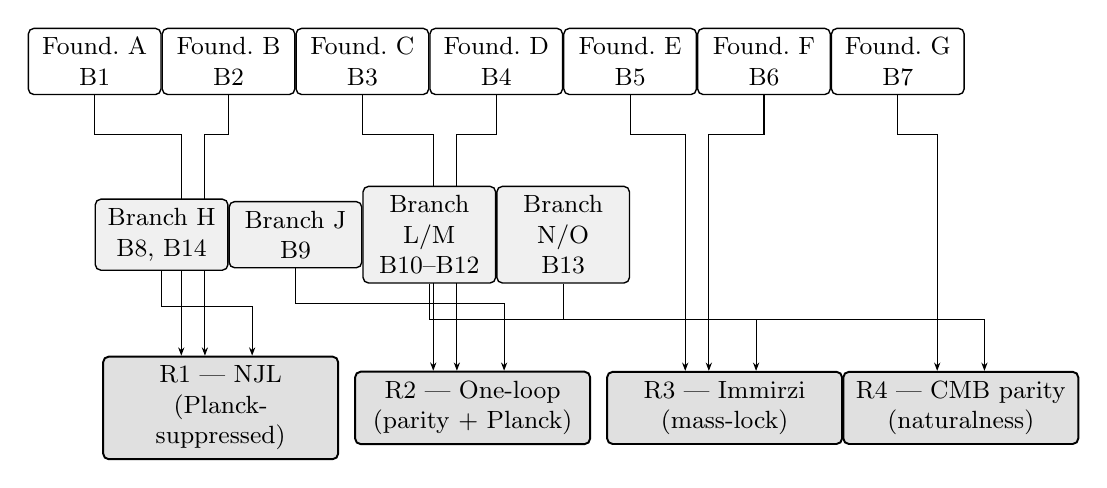
\begin{tikzpicture}[
  font=\small,
  every node/.style={align=center},
  found/.style={draw, rounded corners=2pt, minimum width=1.5cm, minimum height=0.55cm,
                text width=1.45cm, fill=white, draw=black, line width=0.5pt},
  branch/.style={draw, rounded corners=2pt, minimum width=1.5cm, minimum height=0.55cm,
                text width=1.45cm, fill=black!6, draw=black, line width=0.5pt},
  route/.style={draw, rounded corners=2pt, minimum width=2.8cm, minimum height=0.6cm,
                text width=2.75cm, fill=black!12, draw=black, line width=0.7pt},
  arr/.style={-{Stealth[length=3pt]}, black, thin},
]

%% --- Row 1: Foundations A--G ---
\node[found] (A) at ( 0.0, 4.4) {Found.\ A\\B1};
\node[found] (B) at ( 1.7, 4.4) {Found.\ B\\B2};
\node[found] (C) at ( 3.4, 4.4) {Found.\ C\\B3};
\node[found] (D) at ( 5.1, 4.4) {Found.\ D\\B4};
\node[found] (E) at ( 6.8, 4.4) {Found.\ E\\B5};
\node[found] (F) at ( 8.5, 4.4) {Found.\ F\\B6};
\node[found] (G) at (10.2, 4.4) {Found.\ G\\B7};

%% --- Row 3: Closed Routes R1--R4 ---
\node[route] (R1) at ( 1.6, 0.0) {R1 --- NJL\\(Planck-suppressed)};
\node[route] (R2) at ( 4.8, 0.0) {R2 --- One-loop\\(parity $+$ Planck)};
\node[route] (R3) at ( 8.0, 0.0) {R3 --- Immirzi\\(mass-lock)};
\node[route] (R4) at (11.0, 0.0) {R4 --- CMB parity\\(naturalness)};

%% --- Arrows: Foundations -> Routes (drawn before the branch row, so any
%%     crossing segment passes cleanly beneath the branch boxes) ---
\draw[arr] (A.south) -- ++(0,-0.5) -| ([xshift=-0.5cm]R1.north);
\draw[arr] (B.south) -- ++(0,-0.5) -| ([xshift=-0.2cm]R1.north);
\draw[arr] (C.south) -- ++(0,-0.5) -| ([xshift=-0.5cm]R2.north);
\draw[arr] (D.south) -- ++(0,-0.5) -| ([xshift=-0.2cm]R2.north);
\draw[arr] (E.south) -- ++(0,-0.5) -| ([xshift=-0.5cm]R3.north);
\draw[arr] (F.south) -- ++(0,-0.5) -| ([xshift=-0.2cm]R3.north);
\draw[arr] (G.south) -- ++(0,-0.5) -| ([xshift=-0.3cm]R4.north);

%% --- Row 2: Branches H, J, L, M, N, O (grouped into four boxes) ---
\node[branch] (H)  at ( 0.85, 2.2) {Branch H\\B8, B14};
\node[branch] (J)  at ( 2.55, 2.2) {Branch J\\B9};
\node[branch] (LM) at ( 4.25, 2.2) {Branch L/M\\B10--B12};
\node[branch] (NO) at ( 5.95, 2.2) {Branch N/O\\B13};

%% --- Arrows: Branches -> Routes ---
\draw[arr] (H.south)  -- ++(0,-0.45) -| ([xshift=0.4cm]R1.north);
\draw[arr] (J.south)  -- ++(0,-0.45) -| ([xshift=0.4cm]R2.north);
\draw[arr] (LM.south) -- ++(0,-0.45) -| ([xshift=0.4cm]R3.north);
\draw[arr] (NO.south) -- ++(0,-0.45) -| ([xshift=0.3cm]R4.north);

\end{tikzpicture}
\caption{\textbf{Structure of the 14-entry barrier closure.} Top row: the
7 foundation mechanism classes (Foundations A--G; Barriers~1--7,
mechanism-class barriers). Middle row: the 6 observational-channel
branches (Branches H, J, L, M, N, O; Barriers~8--14,
observational-channel barriers), grouped into four boxes --- Branch~H
(B8, B14), Branch~J (B9), Branches~L/M (B10--B12), and Branches~N/O
(B13). Bottom row: the four closed dark-energy routes R1--R4; all four
routes are closed, giving 13 distinct mechanism-class constraints. Arrows
indicate which barrier classes constrain each route. B14 (perturbation
transparency, the ECH perturbation-gate closure) sits in Branch~H and
subsumes B8 (parity-even interaction), so B8 is not counted separately;
several entries share the scaling ansatz but each probes a distinct
physical failure mode.
\label{fig:barrier_map}}
\end{figure*}

\begin{table*}[tb]
\caption{\label{tab:barriers} The 14 catalogue entries (13 distinct mechanism-class constraints;
B8 subsumed by B14) on minimal ECH dark-energy routes. Note: Barriers 8 (parity-even
interaction) and 14 (perturbation transparency) close the same
observable channel (primordial-GW chirality / tensor parity violation)
via related routes sharing the perturbation-transparency result; B14 is the first-principles theorem that
subsumes B8 as the corresponding observational consequence. They are
listed separately to preserve the historical mechanism-class catalog,
but should not be counted as a separate mechanism-class constraint.}
\centering
\begin{tabular*}{\textwidth}{@{\extracolsep{\fill}}clll}
\toprule
\# & Barrier & Source & Mechanism Blocked \\
\midrule
1 & Mass-Coupling Lock & Found.\ A & Propagating torsion as DE \\
2 & Topological-Shift Duality & Found.\ B & Geometric pseudoscalar mass protection \\
3 & Scalar-Tensor Universality & Found.\ C & Distinctive geometric content on FRW \\
4 & Planck Suppression & Found.\ D & Disformal / connection coupling effects \\
5 & Scale Separation & Found.\ E & Global vacuum integral coupling \\
6 & Attractor-Sensitivity Dilemma & Found.\ F & Initial-condition transfer to DE \\
7 & Parameter Immunity & Found.\ G & Cyclic vacuum selection \\
8 & Parity-Even Interaction & Branch H & Tensor chirality from the bounce \\
9 & Liouville Conservation & Branch J & Reversible state selection \\
10 & UV$\to$IR Specificity Dilemma & Branch L & Generic vs.\ bounce-specific bridge \\
11 & Decoupling Universality & Branch L/M & Light gauge field coupling \\
12 & Vacuum Amplification Ceiling & Branch M & Gravitational wave amplitude \\
13 & Gravitational Democracy & Branch N/O & Relics, baryogenesis, vacuum transitions \\
14 & Perturbation Transparency & Branch H (ECH gates) & ECH-specific perturbation signatures \\
\bottomrule
\end{tabular*}
\end{table*}

\subsection{Barrier details}\label{sec:barrier_details}

The fourteen catalog entries of Table~\ref{tab:barriers} are stated compactly
below; the route each barrier constrains is given in brackets (the
barrier$\to$route map is drawn in Fig.~\ref{fig:barrier_map}). The entries
are compact mechanism statements; several (B1, B4, B12) include explicit
order-of-magnitude scaling relations inline.

\medskip\noindent\textbf{B1 --- Mass-Coupling Lock (Found.\ A) [R1].} In Poincar\'{e} gauge
theory (PGT), ultralight torsion modes ($m_T\sim H_0$) require
$g_{\rm eff} \sim 1/(\MPl\sqrt{|t_3|}) \sim H_0/\MPl \sim 10^{-61}$, where $t_3$
is the quadratic-torsion coupling controlling the tensor-torsion mode mass, with
$\sqrt{|t_3|} \sim m_T^{-1}$ for an ultralight mode (a labeled scaling ansatz of
the PGT mass spectrum, not a derived equality). Achieving $g_{\rm eff}\sim 1$
needs $m_T\sim\MPl$; the required tuning
$\delta m_T^2/m_T^2\sim (H_0/\MPl)^2 \sim 10^{-122}$ is the standard
cosmological-constant hierarchy.

\medskip\noindent\textbf{B2 --- Topological-Shift Duality (Found.\ B) [R1].} In metric-affine
gravity, mass protection $\iff$ no geometric fingerprint: configurations
protecting the pseudoscalar mass through topological structure eliminate the
geometric content (the field reduces to a standard ALP after torsion
elimination), while configurations preserving geometric content cannot protect
the mass.

\medskip\noindent\textbf{B3 --- Scalar-Tensor Universality (Found.\ C) [R2].} On an FRW
background, diffeomorphism invariance forces the torsion fluctuation to couple to
the curvature invariants like any other scalar, with no ECH-specific observable;
torsion decouples from the FRW background precisely at the bounce density,
yielding no distinctive perturbation signal.

\medskip\noindent\textbf{B4 --- Planck Suppression (Found.\ D) [R2].} Disformal torsion couplings
are Planck-suppressed by $m_\phi^2/\MPl^2$ or $(\partial\phi)^2/\MPl^4$; at
cosmological scales ($m_\phi\sim H_0$) these are
$\mathcal{O}(10^{-122})$---observationally inaccessible.

\medskip\noindent\textbf{B5 --- Scale Separation (Found.\ E) [R3].} The global vacuum integral
$\int d^4x\,\sqrt{-g}\,\rho_\Lambda$ cannot be connected to the local bounce
density without a mechanism to store and transfer the integrated vacuum energy
across $N_{\rm tot}\approx 92$--$94$ $e$-folds of inflation
(Appendix~\ref{app:dimensions}); none exists within minimal ECH.
(General naturalness/classification argument, not an ECH-specific calculation.)

\medskip\noindent\textbf{B6 --- Attractor-Sensitivity Dilemma (Found.\ F) [R3].} If post-bounce
inflation converges to an attractor, bounce initial conditions are washed out;
if it is sensitive to them, inflation destabilizes. The bounce cannot
simultaneously seed dark energy \textit{and} preserve standard inflation
dynamics. (General naturalness argument.)

\medskip\noindent\textbf{B7 --- Parameter Immunity (Found.\ G) [R4].} Cyclic vacuum selection
requires $\gamma$ to vary across cycles, but $\gamma$ is fixed by the LQG area
spectrum at a universal value; LQG provides no landscape of $\gamma$ values for
selection to operate on. (General classification argument.)

\medskip\noindent\textbf{B8 --- Parity-Even Interaction (Branch H).} \emph{[R1; subsumed by B14.]}
The spin-torsion interaction $(J^5)^2$ is parity-\textit{even} (a product of two
axial currents is a Lorentz scalar, not a pseudoscalar), so it cannot generate
tensor chirality in primordial gravitational waves; independently confirmed by
the perturbation-transparency result (B14).

\medskip\noindent\textbf{B9 --- Liouville Conservation (Branch J) [R2].} Phase-space volume
conservation prevents irreversible selection among post-bounce states, closing
the ``vacuum selection at the bounce'' class: the time-symmetric bounce selects
no net dark-energy state. This is a \emph{heuristic} closure under explicit
assumptions (closed non-dissipative evolution, no particle production, no entropy
injection); dissipative/particle-producing bounces evade B9 and are constrained
instead by B10--B11, so B9 is never used as a stand-alone closure.

\medskip\noindent\textbf{B10 --- UV$\to$IR Specificity Dilemma (Branch L) [R3].} Any bridge from
Planck-scale bounce physics to the late-time $H_0$ scale must be either generic
(explaining \emph{any} vacuum energy) or bounce-specific (requiring free
parameters equivalent to the cosmological constant); no ECH mechanism achieves
both. (General naturalness argument.)

\medskip\noindent\textbf{B11 --- Decoupling Universality (Branches L/M) [R3].} At low energies all
gauge fields decouple from the Planck-suppressed torsion sector equally; the ECH
bounce cannot preferentially couple to photons or dark-energy degrees of freedom
without new non-minimal couplings.

\medskip\noindent\textbf{B12 --- Vacuum Amplification Ceiling (Branch M) [R3].} Gravitational-wave
production from the ECH bounce is bounded above by
$\Omega_{\rm GW}^{\rm ECH}|_{\rm bounce} \lesssim (\rhocrit/\rhoPl)^2 \simeq
0.07\text{--}0.17$, using the LQG-bounce critical-density window
$\rhocrit/\rhoPl \simeq 0.27\text{--}0.41$ from the Ashtekar--Singh effective-LQC
status report~\cite{Ashtekar2011}. The quadratic scaling is an order-of-magnitude
ceiling \emph{ansatz} (not derived here); B12 is used only as a global ceiling.
This bounce-epoch fraction is not directly comparable to the present-day PTA
spectral density $\Omega_{\rm GW}(f_{\rm nHz}) \sim 10^{-9}$ (which differs by
redshift/dilution and by frequency-integration); a quantitative NANOGrav
comparison requires propagating the bounce GW spectrum through the transfer
function to the nHz band, deferred to a dedicated bounce-GW paper, so B12 closes
as a global energy-density-fraction ceiling, not a direct NANOGrav exclusion.

\medskip\noindent\textbf{B13 --- Gravitational Democracy (Branches N/O) [R4].} Torsion couples
democratically to all spin-$1/2$ species and cannot preferentially source
baryogenesis, dark-matter relics, or vacuum transitions without
species-dependent non-minimal couplings. (Structural/philosophical observation,
included for completeness.)

\medskip\noindent\textbf{B14 --- Perturbation Transparency (Branch H, ECH perturbation gates).} \emph{[R1--R4.]} For
canonical scalar matter, torsion vanishes at all perturbation orders and the Holst sector
decouples from all scalar/tensor perturbation observables; elaborated, with the
scalar-sector proof and explicit all-order Holst-term verification, in the
companion paper's zero-spin-branch analysis~\cite{Golden2026P1a}. This is
one of the two first-principles results in the catalog.


%% ============================================================
%%  THE R2/R3 DARK-ENERGY ROUTE CLOSURES
%% ============================================================
\section{The Route-2/Route-3 Dark-Energy Route Closures}\label{sec:routes}

The two routes closed in this section are \emph{historical} candidate
mappings --- one-loop Holst-sector corrections (Route~2) and
Immirzi-parameter running (Route~3) mapped onto a late-time dark-energy
density --- that the companion paper explicitly does not retain as results:
the cited calculations do not derive the required cosmological stress
tensor and observable
matching~\cite{ShapiroTeixeira2014,BenedettiSpeziale2011run}. Nothing in
this section reinstates them. The closures below are upper-bound
\emph{amplitude budgets} demonstrating that any completion of these
mappings falls short of the observed dark-energy density by tens of orders
of magnitude --- which is precisely why the catalog closes the
corresponding channels. The published one-loop inputs enter as
normalization anchors for the budgets, not as derivations of a
cosmological observable.

\subsection{Route 2 (one-loop graviton corrections to the Holst sector):
closed by parity-odd coefficient and Planck suppression}
\label{sec:r2_oneloop}
At the classical level the Holst term $\gamma^{-1}\,e^a\!\wedge e^b\wedge
R_{ab}$ vanishes identically in the torsion-free sector by the first
algebraic Bianchi identity (it is \emph{not} a topological invariant in the
sense of the Pontryagin density; it reduces to the Nieh--Yan density plus a
torsion-squared piece, both of which vanish at $T=0$, as established in the
companion paper's zero-spin-branch analysis~\cite{Golden2026P1a}) and reduces to
the Nieh--Yan density on shell once torsion is integrated out~\cite{Holst1996,Freidel2005}. Quantum
corrections from minimally coupled fermions, however, generate a
parity-odd coupling between the gravitational field and the chiral
fermion current at one loop, with the Holst sector developing
running couplings analyzed via renormalization-group methods in
Einstein--Cartan + Holst gravity~\cite{Mercuri2009,
ShapiroTeixeira2014}. Motivated by (but \emph{not literally
derived in}) the Holst$+$non-minimal-fermion construction of
Mercuri and the one-loop analysis of Shapiro \& Teixeira---those
works establish the classical structure of the Holst term coupled
to fermions, the Nieh--Yan invariant, and the one-loop running of
the Holst sector, not this exact effective operator---we adopt
the phenomenological one-loop parity-odd operator
\begin{equation}
\Gamma_{\rm one\text{-}loop}^{\rm parity\text{-}odd}
= -\,\frac{1}{16\pi^2}\,
\frac{\beta(\gamma)}{M_{\rm Pl}}\,
\int d^4x\sqrt{-g}\,
\partial_\mu\vartheta_{\rm NY}(x)\,J^{5\mu},
\label{eq:oneloop_parity_odd}
\end{equation}
where $\vartheta_{\rm NY}(x)$ is the Nieh--Yan pseudoscalar (mass dimension $+1$; written
$\vartheta_{\rm NY}$ to distinguish it from a photon-sector spectator
ALP $\theta$ of the R4 channel, Sec.~\ref{sec:routes_summary}; no identification
between the two fields is assumed anywhere in this paper), $J^{5\mu}$
is the fermion axial current, and $\beta(\gamma)$ is a slowly varying
function of $\gamma$.\footnote{Parity classification of
Eq.~\eqref{eq:oneloop_parity_odd}. For $\vartheta_{\rm NY}$ a pseudoscalar,
$\partial_\mu\vartheta_{\rm NY}$ transforms as a pseudo-co-vector; $J^{5\mu}$
is also a pseudo-vector; their Lorentz-scalar contraction
$\partial_\mu\vartheta_{\rm NY}\,J^{5\mu}$ is therefore parity-EVEN as a
Lagrangian term. The parity-violating phenomenology in Route 2 arises not
from the operator's intrinsic P transformation but from a P-breaking
\emph{background} expectation $\langle\partial_\mu\vartheta_{\rm NY}\rangle\neq 0$
(the time-dependent cosmological Nieh--Yan pseudoscalar selects a preferred
temporal orientation, spontaneously breaking P and T). The label
``parity-odd'' used in the section heading and surrounding text refers to
the resulting parity-violating phenomenology, not the operator's intrinsic
parity. To avoid ambiguity we therefore read ``parity-odd'' throughout Route~2
(and in the section heading and the superscript of
Eq.~\eqref{eq:oneloop_parity_odd}) strictly as \emph{parity-violating in effect}
via the P-breaking Nieh--Yan background, never as a claim that the Lagrangian
density is P-odd under an unbroken parity transformation; the label is retained
only for continuity with the established Route-2 terminology and carries no
physical content beyond this background-induced parity violation. The photon-coupling chain
used in the dimensionless ratio below proceeds via the standard
chiral-anomaly
$\partial_\mu J^{5\mu} \supset (\alpha_{\rm em}/4\pi)\,F\widetilde F$
relation at the EFT level (the operator above does not itself contain
an electromagnetic field strength); the resulting $\beta$ estimate is
treated strictly as an amplitude-budget bound, not a derived
prediction.} The function
$\beta(\gamma)$ is written with its explicit argument throughout to
distinguish this renormalization-group function from the cosmic
birefringence angle $\beta$ of the R4 channel (Sec.~\ref{sec:routes_summary}). The
coefficient structure of Eq.~\eqref{eq:oneloop_parity_odd} is
\emph{grounded in the explicit one-loop computation} of Shapiro \&
Teixeira~\cite{ShapiroTeixeira2014}, who renormalize on-shell
Einstein--Cartan${+}$Holst gravity with external vector and axial
fermion currents. The parity-odd, Immirzi-dependent current coupling
they renormalize is $\lambda_4=\gamma\,\tilde\kappa^2\,(W\!\cdot\!J)$ (their
Eq.~37; $\tilde\kappa^2\equiv16\pi G\sim M_{\rm Pl}^{-2}$, the imported
convention fixed in Sec.~\ref{sec:conventions}), with classical coefficient
$\alpha_4=-6/(1+\gamma^2)$ and one-loop divergence coefficients
$\Omega_{44}=81\gamma^4/[16(1+\gamma^2)^2]$,
$\Omega_{24}=81\gamma^2/[40(1+\gamma^2)^2]$ (their Eqs.~41--42). Their
master renormalization-group equation $d\lambda/dt=-\sigma/(4\pi)^2$
(their Eq.~46) carries \emph{exactly} the $1/(16\pi^2)$ loop factor
already written in Eq.~\eqref{eq:oneloop_parity_odd}. Three features of
the Route-2 budget are therefore fixed by a published one-loop result
rather than adopted: (i) the loop factor $1/(16\pi^2)$; (ii) the
coefficient $\beta(\gamma)$ is an $\mathcal{O}(1)$ rational function of
the Immirzi parameter [the $\alpha_4$/$\Omega_{4x}$ family, e.g.\
$|\Omega_{44}/\alpha_4|=27\gamma^4/[32(1+\gamma^2)]$, which is
$\mathcal{O}(1)$ for $\gamma\!\sim\!\mathcal{O}(1)$ and
${\approx}2.5\times10^{-3}$ at the LQG value $\gamma\!\approx\!0.24$],
not a free normalization; and (iii) the explicit
$\tilde\kappa^2\sim M_{\rm Pl}^{-2}$ on every renormalized charge, i.e.\ the
Planck suppression in the prefactor $\beta(\gamma)/M_{\rm Pl}$. What the
one-loop analysis does \emph{not} fix is the single \emph{absolute}
normalization: Shapiro \& Teixeira show the coupled flow for
$\lambda_4(t)$ and $\gamma(t)$ (their Eqs.~51,~58) is a Riccati system
whose particular-solution roots are complex for real $\gamma$, so the
Shapiro--Teixeira $\lambda_4$--$\gamma$ system \emph{has no
renormalization-group fixed point} (in contrast to the distinct
Benedetti--Speziale flow of Route~3 below, which has one) and they were
``unable to solve it in a completely satisfactory way.'' A
fully-derived Route-2 amplitude would require a UV boundary condition
plus a controlled solution of that non-perturbative flow (or a
dedicated matching calculation for the exact
$\partial_\mu\vartheta_{\rm NY}J^{5\mu}$ operator). We therefore treat
the \emph{absolute} $\beta(\gamma)$ normalization as a bounded EFT input
while the loop factor, Immirzi-rational coefficient, and Planck
suppression are one-loop-grounded. This is strictly weaker than the
Route-3 result below (whose Benedetti--Speziale $\beta$-function
integrates cleanly to $|\Delta\gamma/\gamma|\approx1.4\times10^{-6}$)
but strictly stronger than a free ansatz: the residual freedom is a
single $\mathcal{O}(1)$ normalization, and the off-shell dimension-$(+1)$
parity-odd operator is in any case bounded by the single-scale NDA no-go
of App.~\ref{app:dimensions} regardless of that $\mathcal{O}(1)$
coefficient, since ST's explicit $\tilde\kappa^2\sim M_{\rm Pl}^{-2}$
confirms the missing powers are Planck powers, not a light scale. Because
the closure below retains ${\approx}\,60$ (conservatively $\geq 58$)
orders of margin, it is insensitive to this residual $\mathcal{O}(1)$
ambiguity in $\beta(\gamma)$.
\emph{Margin note (Eq.~\eqref{eq:oneloop_parity_odd}):} the ${\sim}60$-order
suppression margin renders the precise one-loop prefactor $\beta(\gamma)$
irrelevant to the Route-2 closure: even an $\mathcal{O}(1)$--$\mathcal{O}(10^{10})$
normalization uncertainty leaves $\gtrsim\!48$ orders of amplitude suppression
below the observed birefringence signal, so no plausible prefactor ambiguity
reopens Route~2. The dimensionless coefficient is $\mathcal{O}(\alpha_{\rm em}/4\pi)$
multiplied by the Planck mass to a single negative power. Explicitly, the
prefactor $\beta(\gamma)/M_{\rm Pl}$ carries mass dimension $-1$ (the
division by $M_{\rm Pl}$, not multiplication): with $\vartheta_{\rm NY}$ of
dimension $+1$, $\partial_\mu\vartheta_{\rm NY}$ has dimension $+2$ and the
axial current $J^{5\mu}=\bar\psi\gamma^\mu\gamma^5\psi$ has dimension $+3$,
so the integrand $[\beta(\gamma)/M_{\rm Pl}]\,\partial_\mu\vartheta_{\rm NY}J^{5\mu}$
carries dimension $-1+2+3=+4$ and the action $\int d^4x\sqrt{-g}\,(\cdots)$
is dimensionless, as required. Once
$\partial_\mu\vartheta_{\rm NY} \sim H \sim 10^{-33}\,$eV at the present epoch is
substituted, the induced birefringence accumulated between
recombination and today is, in the dimensionless ratio
$\Delta\theta_{\rm one\text{-}loop}/\Delta\theta_{\rm obs}$,
\begin{align}
\frac{\Delta\theta_{\rm one\text{-}loop}}{\Delta\theta_{\rm obs}}
&\sim \frac{\alpha_{\rm em}}{4\pi}\,\frac{H_0/M_{\rm Pl}}{M_{\rm Pl}\,(\alpha/M)\,\beta_{\rm obs}}\nonumber\\
&\sim \frac{\alpha_{\rm em}}{4\pi}\,\frac{H_0}{M_{\rm Pl}}\,\frac{M}{\alpha\,M_{\rm Pl}\,\beta_{\rm obs}}\,,
\end{align}
where $\alpha_{\rm em}/(4\pi) \approx 5 \times 10^{-4}$ (more precisely $5.8\times 10^{-4}$; the order-of-magnitude closure is robust to this factor), $H_0/M_{\rm Pl} \sim
10^{-61}$, and the R4-fitted coupling $\alpha/M \sim 10^{-21}\,\text{GeV}^{-1}$
(Sec.~\ref{sec:routes_summary}) gives $M_{\rm Pl}\cdot(\alpha/M) \sim 10^{19}\,\text{GeV} \cdot
10^{-21}\,\text{GeV}^{-1} = 10^{-2}$. Plugging in $\beta_{\rm obs}
= 0.342^\circ \approx 6\times 10^{-3}\,\text{rad}$
($0.342\times\pi/180 = 5.97\times 10^{-3}$), the dimensionless ratio is
$\Delta\theta_{\rm one\text{-}loop}/\Delta\theta_{\rm obs} \sim
10^{-3} \cdot 10^{-61}/(10^{-2}\cdot 6\times 10^{-3})\approx 10^{-60}$
(canonical evaluation of the displayed contraction; we conservatively
allow up to two orders of magnitude for unmodeled higher-order
loop-ordering corrections, i.e.\ suppression by at least $10^{-58}$ ---
an explicit conservatism allowance, \emph{not} a derived range; the
$\mathrm{eV}$-vs-$\mathrm{GeV}$ unit conversion is exact
$1\,\mathrm{GeV} = 10^9\,\mathrm{eV}$ and is not a source of
ambiguity), i.e.\ the one-loop induced $\beta$ is suppressed by
${\approx}60$ (conservatively $\geq 58$) orders of magnitude relative
to the observed signal. The qualitative closure is robust to the illustrative
prefactor: even inflating the one-loop coefficient by ten orders of magnitude
leaves ${\gtrsim}\,48$ orders of suppression margin, so no plausible
$\mathcal{O}(1)$--$\mathcal{O}(10^{10})$ normalization ambiguity reopens the
route. We adopt this contraction as the canonical Route-2 estimate;
an alternative ordering that contracts the $H_0$ factor with the
dimensionful coupling differently yields a deliberately loose
$\sim 10^{-33}$ upper bound, not used in the closure.
The canonical-bound conclusion that the one-loop induced $\beta$ is
amplitude-suppressed many orders of magnitude below the observed
WMAP$+$Planck birefringence signal (with ACT~DR6 follow-up) is robust
to this choice; Route~2 remains exploratory framing, not load-bearing
for the no-go. The Route-2 amplitude is
therefore far below not only the WMAP$+$Planck birefringence sensitivity but the
observed central value itself; the one-loop Holst-sector parity-odd
term cannot account for the observed birefringence amplitude. (A naive comparison of a rotation rate $\dot\beta$ in eV against an angle
uncertainty in eV would silently treat $\mathrm{eV}\cdot\mathrm{s}$ as
dimensionless; the dimensionless reduction above avoids this and recovers
the standard R2 amplitude-suppression closure.)
\emph{Closure: amplitude-suppressed by $M_{\rm Pl}^{-1}$ and one-loop
factor $\alpha_{\rm em}/(4\pi)$.}
We stress the status of this estimate explicitly, since it bears directly on the
strength of the no-go: Eq.~\eqref{eq:oneloop_parity_odd} is an \emph{illustrative
upper-bound amplitude budget} constructed as the natural EFT operator at the
$M_{\rm Pl}^{-1}\alpha_{\rm em}/(4\pi)$ scale, \emph{not} a result extracted from
Mercuri~\cite{Mercuri2009} or Date--Kaul--Sengupta~\cite{DateKaulSengupta2009},
which establish the classical Holst/Nieh--Yan structure but not this coefficient.
Because the resulting suppression carries a margin of ${\sim}60$ orders of
magnitude, the qualitative closure is insensitive to the precise coefficient: even
inflating the ansatz prefactor by $\mathcal{O}(1)$--$\mathcal{O}(10^{10})$ (far
beyond any plausible EFT enhancement) still leaves the induced $\beta$ tens of
orders of magnitude below the observed signal. The Route-2 amplitude-budget
closure is therefore
robust to the ansatz-level status of the operator, and we present it as an
amplitude-budget bound rather than a rigorous derivation. The same logic applies
to Route~3 below.

\subsection{Route 3 (quantum running of the Immirzi parameter):
closed by mass-dimension lock}
\label{sec:r3_immirzi}
A second route to a parity-odd ECH contribution is the quantum running
of the Barbero--Immirzi parameter $\gamma$ itself. Date, Kaul \& Sengupta
analyzed the Holst term coupled to fermions and the Nieh--Yan
invariant in the chiral-matter setting~\cite{DateKaulSengupta2009};
that analysis establishes a topological interpretation of $\gamma$
and motivates a $\gamma$-running in the presence of chiral asymmetry,
but does \emph{not} itself present the explicit RG equation used
below. Schematically motivated by their construction, we adopt the
one-loop running ansatz
\begin{equation}
\frac{d\gamma}{d\ln \mu}
= \frac{1}{12\pi^2}\,(N_F^L - N_F^R) \, \gamma + \mathcal{O}(\gamma^2),
\label{eq:gamma_running}
\end{equation}
where $N_F^L$ and $N_F^R$ are the numbers of left- and right-chiral
Weyl fermions running in the loop. The $1/(12\pi^2)$ prefactor is
the natural chiral-loop coefficient at this order; we use
Eq.~\eqref{eq:gamma_running} only as an upper-bound EFT ansatz
for the Route-3 amplitude budget and do not claim it is taken
verbatim from~\cite{DateKaulSengupta2009}. The actual fermion-induced
perturbative running of the Immirzi parameter is computed by
Benedetti~\&~Speziale~\cite{Benedetti2011}, who find a $\beta$-function
whose sign depends on $|\gamma|$ through four-fermion interactions
generated when fermions are coupled to the Holst sector; our
Eq.~\eqref{eq:gamma_running} is a chiral-count EFT bound rather than
the full perturbative result, and is used solely for the amplitude
budget below. We can, moreover, do better than an estimate. The actual fermion-coupled
one-loop $\beta$-function was computed by Benedetti \&
Speziale~\cite{BenedettiSpeziale2011run} (their Eq.~7),
\begin{equation}
\mu\,\frac{\partial\gamma^2}{\partial\mu}
= -(\gamma^2-1)\,\frac{\mu^2\tilde\kappa^2}{(8\pi)^2}\,(23\gamma^2+5),
\qquad \tilde\kappa^2 \equiv 16\pi G,
\label{eq:bs_beta}
\end{equation}
whose only fixed point (of this Benedetti--Speziale flow; the
fixed-point-free Riccati system above is Shapiro--Teixeira's Route-2
$\lambda_4$--$\gamma$ system, a different flow) is the
ultraviolet-attractive $\gamma^2=1$
(formally outside perturbative control), with the sign of the flow set by
whether $|\gamma|\gtrless 1$ and the running driven by the
radiatively-generated four-fermion interaction. The decisive feature is
the explicit $\mu^2\tilde\kappa^2\simeq(\mu/M_{\rm Pl})^2$ prefactor: the running is
\emph{power-suppressed} by the renormalization scale in Planck units, not
logarithmic, so the accumulated $\int\!\beta_{\gamma^2}\,d\ln\mu \propto
\int\!\mu\,d\mu$ is dominated by the ultraviolet endpoint and is of order
$(\mu_{\rm UV}/M_{\rm Pl})^2$. Integrating Eq.~\eqref{eq:bs_beta}
numerically from a GUT-scale ultraviolet boundary
$\mu_{\rm UV}\sim10^{16}\,$GeV down to $\mu_{\rm IR}\sim1\,$GeV (with
$\gamma$ near the LQG value $\gamma\!\approx\!0.24$) gives, in agreement
with a frozen-coefficient analytic estimate to four significant figures,
$|\Delta\gamma/\gamma|\approx1.4\times10^{-6}$. This is a genuine integrated
running, \emph{not} an ansatz bound: the explicit
$\mu^2\tilde\kappa^2\simeq(\mu/M_{\rm Pl})^2$ prefactor makes the flow power-suppressed,
so $|\Delta\gamma/\gamma|\sim(\mu_{\rm UV}/M_{\rm Pl})^2$ and the integral is
dominated by the ultraviolet endpoint. The result is perturbatively
controlled for any sub-Planckian UV boundary; only a literal Planck-scale
boundary would push $|\Delta\gamma/\gamma|\to\mathcal{O}(1)$, precisely the
regime Benedetti \& Speziale flag as outside perturbative control (the
$\gamma^2=1$ fixed point corresponds to a divergent four-fermion coupling),
so a Planck-scale evaluation would require UV-completion input beyond the
one-loop $\beta$-function. The derived physical running therefore only
\emph{strengthens} Route~3, and this GUT-UV integrated value is the
primary Route-3 estimate. Propagated to the dark-energy channel through the paper's own
$(\Delta\gamma/\gamma)\cdot(H_0/M_{\rm Pl})$ mass-dimension suppression, the
derived torsion/Immirzi contribution to $\rho_\Lambda$ sits
$\sim 61$--$67$ orders of magnitude below the observed dark-energy density
$\rho_{\Lambda,\rm obs}\approx(2.25\,\text{meV})^4$ --- so the no-go closes
with enormous margin, now from a \emph{derived} integrated result rather
than an ansatz upper bound. We nonetheless retain the far larger
chiral-count estimate Eq.~\eqref{eq:gamma_running},
$\Delta\gamma/\gamma\!\sim\!0.3$, as a deliberately pessimistic \emph{upper}
bound in the budget below. Because the Route-3
closure below carries $\gtrsim 60$ orders of suppression margin, it is
in any case insensitive to the precise coefficient. In the Standard Model, the chiral
asymmetry is generated by the $SU(2)_L$ doublets. Integrating
Eq.~\eqref{eq:gamma_running} over the running gives
$\Delta\gamma/\gamma \approx (N_F^L-N_F^R)\,
\ln(\mu_{\rm GUT}/\mu_{\rm IR})/(12\pi^2)$; with a net chiral count
$(N_F^L-N_F^R)=\mathcal{O}(1)$ and a GUT-to-IR lever arm
$\ln(\mu_{\rm GUT}/\mu_{\rm IR})\approx 30$--$37$
($\mu_{\rm GUT}\sim 10^{16}$, $\mu_{\rm IR}\sim 1\,\text{GeV}$,
$\ln 10^{16}\approx 36.8$),
this is numerically $\Delta\gamma/\gamma \approx 0.25$--$0.31$
(a few$\,\times 10^{-1}$; e.g.\ $32/(12\pi^2)\approx 0.27$).
We therefore adopt the larger $\Delta\gamma/\gamma \sim 0.3$ as the
\emph{conservative} (least-suppressed) order-of-magnitude estimate ---
\emph{not} a precisely derived value, but a conservative upper bound
consistent with the $|\gamma|$-dependent Benedetti--Speziale
$\beta$-function structure recorded above (four-fermion-driven, sole
fixed point at $\gamma^2=1$, sign set by $|\gamma|\gtrless 1$) ---
and note that the Route-3
closure below is insensitive to its precise value: even this
$\mathcal{O}(0.3)$ running is $\ll 1$, so $\gamma$ retains its order of
magnitude, and it still leaves $\gtrsim 60$ orders of suppression margin. The Holst sector amplitude that this running can source is
fixed by mass dimension: any operator built from
$\gamma$, $R_{ab}$, $e^a$, and the chiral current $J^{5\mu}$ must carry
dimension four, which forces a single power of $M_{\rm Pl}^{-1}$ in
the prefactor in any cosmologically relevant scalar-curvature regime.
Plugging the conservative $\Delta\gamma/\gamma \sim 0.3$ into the resulting
parity-odd amplitude, the cosmologically integrated effect is
suppressed by an additional factor of
$(\Delta\gamma/\gamma)\cdot(H/M_{\rm Pl}) \sim 3\times 10^{-62}$ relative to
the dimensionless parity-odd amplitude budget associated with a
dark-energy-scale source, closing this route by many orders of
magnitude. \emph{Closure: mass-dimension-locked at the classical level
and amplitude-suppressed by the chiral-asymmetry running coefficient.}
\emph{Ansatz vs derivation (R2/R3):} R3's magnitude is now a
\emph{derived integrated result}: for a sub-Planckian (GUT-scale) UV
boundary the verified Benedetti--Speziale one-loop $\beta$-function
Eq.~\eqref{eq:bs_beta} integrates to $|\Delta\gamma/\gamma|\approx
1.4\times10^{-6}$, replacing the prior chiral-count ansatz upper bound as
the primary Route-3 estimate. R2's amplitude coefficient is now
\emph{one-loop-grounded}: its loop factor $1/(16\pi^2)$,
$\mathcal{O}(1)$ Immirzi-rational coefficient, and
$\tilde\kappa^2\sim M_{\rm Pl}^{-2}$ Planck suppression are fixed by the Shapiro
\& Teixeira~\cite{ShapiroTeixeira2014} one-loop renormalization of the
Holst${+}$fermion sector (their Eqs.~41--42,~46); only the single
absolute normalization remains a bounded EFT input, because the
Shapiro--Teixeira $\lambda_4$--$\gamma$ flow has no fixed point and is
not perturbatively solvable in closed form, and the operator is bounded by the single-scale
NDA no-go regardless of that $\mathcal{O}(1)$ normalization. The kept ansatz value
Eq.~\eqref{eq:gamma_running} ($\Delta\gamma/\gamma\sim0.3$) is retained
only as a deliberately pessimistic upper bound; the closures of R2/R3
survive an $\mathcal{O}(1)$ inflation of the ansatz coefficient because
the resulting amplitude suppression ($\sim 3\times 10^{-62}$ vs
$\rho_\Lambda$, using the pessimistic $\Delta\gamma/\gamma \sim 0.3$)
leaves $\gtrsim 60$ orders of magnitude of margin against any
$\mathcal{O}(1)$ rescaling of the chiral-asymmetry coefficient, and the
derived $1.4\times10^{-6}$ value only widens that margin.
\emph{Strict theoretical limitation:} the NDA one-loop operator (R2) and
Immirzi-running (R3) inputs used here are bounded EFT inputs, not UV-complete
flow derivations---the R2 absolute normalization requires a controlled solution
to the ST Riccati system (no real fixed point; ST explicitly state they could
not solve it satisfactorily), and the R3 chiral-count
Eq.~\eqref{eq:gamma_running} is an order-of-magnitude ansatz rather than the
full Benedetti--Speziale four-fermion-driven RG flow at all loop orders.
These represent the strict theoretical limitation of the R2/R3 analysis within
current loop-gravity technology; the ${\approx}\,58$--$60$-order (and larger) closure margins make
the qualitative conclusions robust to this limitation, but the inputs cannot be
promoted to precision derivations without a UV-complete treatment of the coupled
Holst$+$fermion RG system.

\subsection{The fourth channel and the combined closure}\label{sec:routes_summary}

The fourth enumerated channel, R4, is a direct parity-odd coupling between
the electromagnetic field and a spectator axion-like field or the fermion
axial current, $\mathcal{L}_{\rm CS}\supset
-\tfrac14(\alpha/M)\,\phi\,\widetilde F_{\mu\nu}F^{\mu\nu}$, producing a
rotation of the CMB polarization plane (cosmic birefringence). Fitting
this coupling to the observed WMAP$+$Planck birefringence signal
$\beta_{\rm obs}=0.342^\circ\pm0.094^\circ$~\cite{Minami2020,Eskilt2022}
(comparable to the independent ACT~DR6 measurement
$\beta=0.215^\circ\pm0.074^\circ$~\cite{DiegoPalazuelos2025}) gives the anchor value
$\alpha/M\sim10^{-21}\,\text{GeV}^{-1}$ used above as a numerical input to
the Route-2 amplitude estimate. R4 does not close by amplitude
suppression: the same coupling that reproduces $\beta_{\rm obs}$ can, with
a free normalization, also be tuned to reproduce $\rho_\Lambda$, but
minimal ECH does not derive either the required ultralight mass
$m_\theta\sim H_0$ or the fitted $\alpha/M$ from first principles---so the
channel closes as a naturalness/explanatory-deficit objection (it
relocates rather than solves the cosmological-constant problem) rather
than as an amplitude exclusion. Its full derivation, and the companion
consistency check against a spectator-ALP birefringence benchmark, are
outside the present survey's scope~\cite{Golden2026P1a,Golden2026P1b}.

Within the four-channel enumeration of Sec.~\ref{sec:conventions},
Routes R1--R4 cover the four parity-odd/dark-energy channels of this
framework. Two operators occasionally raised as omissions from this
four-channel enumeration --- the Jackiw--Pi gravitational Chern--Simons
term $R\!\wedge\!\widetilde R$ and the parity-odd four-fermion partner of
R1 carrying the $\gamma_{\rm BI}/(\gamma_{\rm BI}^2{+}1)\cdot 8\pi G$
coefficient --- are closed in the companion analysis~\cite{Golden2026P1a}
(total derivative for constant coupling and R4-class otherwise, for the
Jackiw--Pi term; Planck suppression plus vanishing mean field, inheriting
R1, for the four-fermion partner); the dimension-6 parity-odd
four-fermion basis is Fierz-closed and uniformly Planck-suppressed by the
projection lemma of Appendix~\ref{app:fierz}, so only a non-minimal
completion lies outside the established no-go. Within the four
enumerated channels: R1 (NJL contact) is amplitude-suppressed by
$M_{\rm Pl}^{-2}$ and parity-even. R2 (one-loop graviton corrections) is
amplitude-suppressed by $M_{\rm Pl}^{-1}$ and the one-loop factor
$\alpha_{\rm em}/(4\pi)$. R3 (Immirzi running) is mass-dimension-locked
and additionally suppressed by the chiral-asymmetry beta function. R4
(parity-odd CMB coupling) is closed by a naturalness objection: with
$\alpha/M$ treated as a free parameter, a spectator-ALP fit reproduces
both $\beta_{\rm obs}$ and $\rho_\Lambda$, but minimal ECH does not
derive $m_\theta\sim H_0$ or the fitted $\alpha/M$, so the channel closes
at the level of an explanatory deficit rather than an amplitude
exclusion.

\emph{Tiered closure structure:} R1--R3 achieve \emph{mathematical
amplitude closure} (the predicted amplitude is suppressed by explicit
$M_{\rm Pl}$ powers and loop factors, placing it many orders below any
observable threshold regardless of normalisation assumptions);
R4 achieves \emph{naturalness/explanatory closure} (the amplitude can
be matched to observations but only at the cost of importing the
cosmological-constant fine-tuning the channel was meant to resolve).
These are logically distinct closure modes and are classified
separately in the evidentiary table below.

\paragraph{Evidentiary status of each leg.} So that the strength of
the closure is not overread, we state explicitly the evidentiary level
at which each route and each structural result is established. We use a
three-tier scale: \textbf{(I)~rigorous result} --- a deductive
consequence of stated equations/identities, holding exactly within an
explicitly bounded scope; \textbf{(II)~structural argument} --- a
qualitative or order-of-magnitude argument from established physics
(symmetry, parity, naturalness) that does not turn on a fitted number;
and \textbf{(III)~ansatz-level dimensional estimate} --- an
amplitude budget evaluated under an explicitly-labeled scaling ansatz,
honest to a factor but not a first-principles derivation.
Table~\ref{tab:evidentiary_status} classifies every leg on this scale.
No leg is claimed at a level higher than this table records: in
particular, the only Tier-I (rigorous) leg is the
perturbation-transparency result for canonical scalar matter; R2--R3 are
Tier-III ansatz-level estimates; and the R4 closure is a Tier-II
\emph{naturalness/explanatory-deficit} objection, \emph{not} an amplitude
exclusion and conditional on the on-shell scaling ansatz of
Appendix~\ref{app:dimensions}. The aggregate ``four-route channel-level
closure'' is therefore exactly that: a channel-level (not operator-level)
statement whose individual legs sit at the levels tabulated, reinforced
but not promoted by the mechanism-class catalog of
Sec.~\ref{sec:barriers}.

\begin{table*}[tb]
\caption{\label{tab:evidentiary_status} Evidentiary status of each closure
leg, on the three-tier scale of the text: (I)~rigorous result within
stated scope, (II)~structural argument, (III)~ansatz-level dimensional
estimate. The table records the highest level at which each leg is
claimed; no leg is asserted more strongly elsewhere. ``Rules
out'' is to be read at channel-amplitude granularity, not as an
operator-level theorem.}
\begin{ruledtabular}
\begin{tabular}{lll}
\textbf{Leg} & \textbf{What it rules out (channel-amplitude level)} &
\textbf{Evidentiary status} \\
\colrule
\parbox[t]{0.18\textwidth}{\raggedright Perturbation transparency
(companion paper~\cite{Golden2026P1a})\strut} &
\parbox[t]{0.40\textwidth}{\raggedright The Holst sector / Barbero--Immirzi
parameter contributing to scalar or tensor perturbation observables, for
canonical scalar matter\strut} &
\parbox[t]{0.32\textwidth}{\raggedright \textbf{(I) Rigorous} within stated
scope: $T=0$ follows from zero scalar spin density, and the Holst dual
contraction vanishes by the algebraic Bianchi identity. Excludes
propagating-torsion, fermion-loop, dynamical-Immirzi, non-minimal-matter
sectors.\strut} \\[3pt]
\parbox[t]{0.18\textwidth}{\raggedright R1 (NJL four-fermion contact)\strut} &
\parbox[t]{0.40\textwidth}{\raggedright The torsion-induced contact term
sourcing coherent $w\!=\!-1$ dark energy\strut} &
\parbox[t]{0.32\textwidth}{\raggedright \textbf{(II)+(III)}: parity-even
structure ($\langle J^5\rangle\!\approx\!0$, no coherent mean field) is a
Tier-II algebraic fact; the $M_{\rm Pl}^{-2}$ amplitude suppression
(${\sim}70$ orders below $\rho_\Lambda$) is a Tier-III order-of-magnitude
estimate from a standard Cartan torsion-elimination derivation.\strut} \\[3pt]
\parbox[t]{0.18\textwidth}{\raggedright R2 (one-loop graviton
corrections)\strut} &
\parbox[t]{0.40\textwidth}{\raggedright One-loop promotion of
$\gamma_{\rm BI}$ reaching the observed birefringence amplitude\strut} &
\parbox[t]{0.32\textwidth}{\raggedright \textbf{(III) Ansatz-level}: amplitude
budget suppressed by $H_0/M_{\rm Pl}$ and $\alpha_{\rm em}/(4\pi)$ under an
explicitly-labeled scaling ansatz; exploratory, not load-bearing.\strut}
\\[3pt]
\parbox[t]{0.18\textwidth}{\raggedright R3 (Immirzi running)\strut} &
\parbox[t]{0.40\textwidth}{\raggedright Quantum running of $\gamma_{\rm BI}$
generating a dark-energy-relevant shift\strut} &
\parbox[t]{0.32\textwidth}{\raggedright \textbf{(II)+(III)}: mass-dimension
lock is structural; the chiral-asymmetry beta-function bound
(Benedetti--Speziale) is a Tier-III order-of-magnitude upper bound,
deliberately loose and non-load-bearing ($\gtrsim 60$ orders of
margin).\strut} \\[3pt]
\parbox[t]{0.18\textwidth}{\raggedright R4 (parity-odd CMB / spectator-ALP
coupling)\strut} &
\parbox[t]{0.40\textwidth}{\raggedright Minimal ECH \emph{deriving} the single
coupling that yields both $\beta_{\rm obs}$ and $\rho_\Lambda$\strut} &
\parbox[t]{0.32\textwidth}{\raggedright \textbf{(II) Structural naturalness
objection}, \emph{not} an amplitude exclusion: a free-$\alpha/M$ ALP fit
reproduces $\beta_{\rm obs}$, but ECH supplies neither $m_\theta\!\sim\!H_0$
nor the fitted $\alpha/M$, relocating the CC problem. Conditional on the
on-shell scaling ansatz (App.~\ref{app:dimensions}).\strut} \\
\end{tabular}
\end{ruledtabular}
\end{table*}

The phenomenological parameter $\alpha/M$ introduced above is therefore
best understood as the R4-bounded coupling required to
match $\beta_{\rm obs}$, with the dark-energy density supplied by an
unrelated sector (e.g.\ a quintessence field~\cite{Carroll1998}, a
quintom-class two-field scenario~\cite{Cai2010quintomReview}, or by a positive
cosmological constant), rather than by ECH-internal physics. This
inversion of the prior mass-coupling lock is a core structural
finding reused throughout this catalog.

%% ============================================================
%%  THE OPERATOR-BASIS-COMPLETENESS ARGUMENT
%% ============================================================
\section{The Operator-Basis-Completeness Argument}\label{sec:completeness}

The barrier catalog and the Route-2/Route-3 closures above bound the
amplitude of \emph{one} representative parity-odd operator. A referee may
reasonably ask whether the same conclusion survives once the full local
operator basis is considered. This section answers that question: we
exhibit the finite basis of local, gauge-invariant, diffeomorphism-covariant
parity-odd densities of mass dimension exactly four admitted by the
minimal-ECH field content under the construction rule stated below, and show
that the single-scale dimensional bound applies to every member of that
basis, not to one representative.

As a phenomenological ansatz for a direct parity-odd curvature coupling ---
motivated by, but not literally derived from, the Holst-plus-non-minimal-fermion
construction of Mercuri~\cite{Mercuri2009} --- consider the parity-odd term
\begin{equation}\label{eq:Seff}
S_{\rm eff} = \frac{\alpha}{M}\int e_I\wedge e_J\wedge \mathcal{F}^{IJ}[K,\mathring{R}],
\end{equation}
where $M = M_{\rm area\text{-}gap}\sim\MPl/\sqrt{\gamma}$ is the LQG area-gap
mass scale (from the LQG area-gap $\Delta \propto \gamma\,\ell_P^2$, the
inverse-length / mass scale is $M_\Delta \sim M_{\rm Pl}/\sqrt{\gamma}$ up
to numerical constants), $\alpha$ is a dimensionless coupling, and
$\mathcal{F}^{IJ}[K,\mathring{R}]$ denotes the curvature two-form of the
full (torsionful) connection, written as a functional of the contorsion
$K$ and the Levi-Civita curvature $\mathring{R}$; the component form
Eq.~(\ref{eq:Seff_comp}) displays its leading contribution.

In components, the leading contribution reduces to
\begin{equation}\label{eq:Seff_comp}
S_{\rm eff} = \int d^4x\,\sqrt{-g}\;\frac{\alpha}{M}\;\varepsilon^{\mu\nu\rho\sigma}\,e^I_\mu\,e^J_\nu\,\mathcal{F}_{IJ\rho\sigma},
\end{equation}
which has naive mass dimension $[\mathcal{L}_{\rm odd}] = +1$---three units
short of the required $+4$ (with $[\alpha]=0$, $[M]=+1$, $[e^I_\mu]=0$, and
$[\mathcal{F}_{IJ\rho\sigma}]=+2$, the integrand carries mass dimension
$-1+2=+1$). We state this off-shell mismatch deliberately, and we address it
immediately by identifying the physical foundation before using the shorthand.

\emph{Physical foundation: the dimension-$4$ off-shell operator basis.}---The
formally dimension-$4$, gauge-invariant, diffeomorphism-covariant off-shell
operator basis is the closed local expansion
\begin{equation}\label{eq:Seff_dim4}
S_{\rm eff}^{(4)} = \int d^4x\,\sqrt{-g}\sum_{n} c_n\,\mathcal{O}_n^{[4]},
\qquad \{\mathcal{O}_n^{[4]}\}=\{\mathrm{O1}\text{--}\mathrm{O6}\},
\end{equation}
where each $\mathcal{O}_n^{[4]}$ is a genuine dimension-$4$ Lagrangian
density and each Wilson coefficient $c_n$ is a dimensionless rational.
The operators $\{$O1--O6$\}$ constitute the \emph{primary physical
foundation} of the no-go: the single-scale NDA ceiling, the Fierz closure,
and the Bianchi-vanishing results below are all derived properties of this
off-shell dimension-$4$ basis; none depends on the on-shell shorthand
Eq.~\eqref{eq:Seff_comp} for its logical force.
\emph{Construction rule.}---The admitted building blocks are the tetrad
$e^I_\mu$ (with the invariant tensors $\varepsilon$ and $\eta$), the
curvature two-form of the torsionful connection, the algebraically-fixed
torsion $T=\kappa S$, and the minimal axial current $J^5$; densities are
formed at zero additional derivative order (no derivatives beyond those
internal to $R$ and $T$), with a parity-odd $\varepsilon$ contraction,
full index contraction to a scalar density, and mass dimension exactly
four after the explicit $\MPl^{2}$ promotions of
Eq.~\eqref{eq:dim4_defs}. Under this rule the basis is the six-member set
of Eq.~\eqref{eq:dim4_defs}. Completeness of the list is asserted from
the construction rule --- we know of no admitted contraction outside it
--- and is not established by an exhaustive symbolic enumeration; the
released script verifies the two reduction identities used below, not the
enumeration itself.
Because the underlying schematic invariants carry different naive
dimensions under the paper's conventions ($[e]=0$, $[R]=+2$, physical
torsion $[T]=[\kappa S]=+1$, spin current $[S]=[J^5]=+3$,
$[\kappa]=[\MPl^{-2}]=-2$), the operator \emph{definitions} include the
explicit compensating $\MPl$ power that renders each density dimension-$4$;
we do \emph{not} attach a dimensionless $c_n$ to a lower-dimension
invariant.
\emph{Shorthand and its relation to the basis.}---Eq.~\eqref{eq:Seff_comp}
with its dimension-$+1$ integrand is a phenomenological on-shell
representative of the dimension-$4$ basis in which the coefficient
$\alpha/M$ (mass dimension $-1$) stands in for the basis operators'
$\MPl^{2}$ prefactor (mass dimension $+2$) --- exactly the three-unit
coefficient substitution quantified in Appendix~\ref{app:dimensions}; it
is a convenient dimensional-analysis shorthand, \emph{not} the
fundamental action term and \emph{not} load-bearing for the no-go. To
clarify the mass-dimension bookkeeping: the off-shell operators O1--O6 are
genuinely dimension $+4$ (each carrying the compensating $\MPl^2$ factor that
makes the Wilson coefficient dimensionless), while Eq.~\eqref{eq:Seff_comp}
represents the same physics on the torsion-free branch with the
phenomenological coefficient $\alpha/M$ in place of the basis prefactor
$\MPl^{2}$; the apparent dimension-$+1$ deficit is entirely that
$\alpha/M$-for-$\MPl^{2}$ coefficient substitution
(Appendix~\ref{app:dimensions}), not any ill-defined operator. The Case~II on-shell curvature dressing
(inserting $R\sim\MPl^2$ to close the dimension count) is an
\emph{illustrative heuristic}, subordinate to the operator basis and used
solely for dimensional-analysis aesthetics; it carries no independent
logical weight in the no-go argument.
Concretely, the six dimension-$4$ densities are (names as in
Table~\ref{tab:dim4_parityodd})
\begin{align}\label{eq:dim4_defs}
\mathcal{O}_{1}^{[4]}&=\MPl^{2}\,\varepsilon\,e^I e^J R_{IJ},
& \mathcal{O}_{2}^{[4]}&=\MPl^{2}\,\mathrm{NY},\notag\\
\mathcal{O}_{3}^{[4]}&=R^{IJ}\!\wedge R_{IJ},
& \mathcal{O}_{4}^{[4]}&=\MPl^{2}\,\varepsilon_{IJKL}T^{IJ}T^{KL},\notag\\
\mathcal{O}_{5}^{[4]}&=\varepsilon\,T\,e\,J^5,
& \mathcal{O}_{6}^{[4]}&=\MPl^{2}\,\varepsilon^{\mu\nu\rho\sigma}R_{\mu\nu\rho\sigma},
\end{align}
so that Pontryagin (O3, $[R\wedge R]=+4$) and axial--torsion
(O5, $[TeJ^5]=+1+0+3=+4$) already sit at dimension $4$ with a bare
dimensionless coefficient, while the Holst dual, Nieh--Yan, torsion-square,
and single-curvature densities (each of naive dimension $+2$ as component
densities) are promoted to dimension $4$ by the single available scale
$\MPl^{2}$ inside the operator definition. This bookkeeping is essential:
labelling the bare invariants as ``dimension-$4$ with dimensionless $c_n$''
would misstate their mass dimension, whereas the definitions above carry the
$\MPl^{2}$ prefactors explicitly so that every
$c_n\mathcal{O}_n^{[4]}$ is a bona-fide dimension-$4$ density. The physics
conclusion is unchanged: the algebraic Cartan constraint $T=\kappa S$, the
first (algebraic) Bianchi identity, and Chern--Weil exactness collapse this
set to (i) topological total derivatives (O2, O3), (ii) the
$\MPl^{-2}$-suppressed Fierz-closed four-fermion sector (O4, O5), or
(iii) Bianchi-vanishing single-curvature densities (O1, O6).

\emph{Main-text completeness argument.}---The collapse is closed by the
exhibited finite basis plus two tensor identities; the identities are
verified symbolically in the released script
\texttt{arxiv/scripts/dim4\_parityodd\_enumeration.py} (the script
verifies the two identities, not the enumeration, which rests on the
construction rule above). (a) The single-curvature
parity-odd densities vanish identically: for any Riemann tensor obeying the
pair antisymmetries and the algebraic Bianchi identity $R_{\mu[\nu\rho\sigma]}=0$,
$\varepsilon^{\mu\nu\rho\sigma}R_{\mu\nu\rho\sigma}=0$, killing both O1 and O6
on the torsion-free branch. (b) The torsion-square and axial--torsion densities
reduce under $T=\kappa S$, using
$S_{abc}S^{abc}=-\tfrac38\,(J^5\!\cdot\!J^5)$ (from $S^{abc}=\tfrac14\varepsilon^{abcd}J^5_d$ and the
Lorentzian $\varepsilon_{abcd}\varepsilon^{abce}=-3!\,\delta^e_d$, consistent with the
companion paper's torsion-elimination normalization~\cite{Golden2026P1a}), to the parity-odd
four-fermion contact operator $\kappa^{2}(J^5\!\cdot\!J^5)$, which the
Fierz-by-Fierz projection lemma (Appendix~\ref{app:fierz}) shows closes onto
the finite $\{SS,VV,AA,PP\}$ basis with \emph{no} escape operator and \emph{no}
change of $\MPl^{-2}$ power. (c) O2 (Nieh--Yan) and O3 (Pontryagin) are exact
total derivatives, contributing zero to the local equations of motion and zero
to the vacuum energy. Hence every admissible local dimension-$4$ parity-odd
density in minimal ECH is topological, Fierz-basis-reducible, or
Bianchi-vanishing, and none produces a $(\text{meV})^4$ vacuum energy without a
new light scale $\mu\ll\MPl$ or a protected symmetry --- either of which is
itself the tuning to be explained. The concrete operator definitions, the
symbolic checks, and the Fierz matrix are given in full in
Appendices~\ref{app:dim4_completion}--\ref{app:fierz}
(Table~\ref{tab:dim4_parityodd}). On the on-shell branch (algebraic torsion eliminated; O1/O6 vanishing
identically by the algebraic Bianchi identity, O2/O3 total derivatives),
this closed dimension-$4$ set is represented by the single dimension-$+1$
shorthand of Eq.~\eqref{eq:Seff_comp}, whose coefficient $\alpha/M$
(dimension $-1$) replaces the basis operators' $\MPl^{2}$ prefactor
(dimension $+2$): the $+1$-vs-$+4$ counting is exactly that three-unit
coefficient substitution (Appendix~\ref{app:dimensions}), not a property
of an ill-defined action.
The identification $\rho_\Lambda = \Xi\,\MPl^4$ is therefore governed by a
\textit{single-scale NDA dimensional no-go} that holds identically for the
formal dimension-$4$ basis and its dimension-$+1$ shorthand
(Appendix~\ref{app:dim4_completion} verifies the closure survives at genuine
dimension~$4$ without the on-shell dressing): the three-unit deficit forces
the missing powers to $\MPl^3$ (the only scale in minimal ECH), so the
natural density is $\sim\MPl^4$, never $(\text{meV})^4$
(Appendix~\ref{app:dimensions}). This is a dimensional-impossibility
argument, not a derived amplitude, and hence not circular; it is treated as
such throughout.

%% ============================================================
%%  DISCUSSION: SCOPE AND BOUNDARIES
%% ============================================================
\section{Discussion: Scope and Boundaries}\label{sec:scope}

Consistent with the evidentiary classification of Sec.~\ref{sec:barriers}
and Table~\ref{tab:evidentiary_status}, we state explicitly what this
survey does and does not establish.

\emph{What is established.} Thirteen distinct mechanism-class constraints,
covering seven foundational classes and six observational branches,
collectively close the four enumerated minimal-ECH dark-energy channels
(R1--R4) under stated assumptions. Two of those channels (R2, R3) are
closed here at the amplitude-budget level with margins of order sixty
(conservatively $\geq 58$) orders of magnitude; the closures are robust to
$\mathcal{O}(1)$--$\mathcal{O}(10^{10})$
rescalings of their ansatz-level normalizations. The operator-basis-completeness
argument (Sec.~\ref{sec:completeness}) extends the governing dimensional bound
from one representative operator to the exhibited six-member local
dimension-four parity-odd operator basis $\{$O1--O6$\}$ admitted by the
minimal-coupling field content, with no escape operator identified within
that basis; completeness of the basis is asserted from the stated
construction rules, not proved by exhaustive symbolic enumeration.

\emph{What is not established.} This is a \emph{channel-level}, not a fully
operator-level, no-go over the entire space of diffeomorphism-invariant
gravitational operators: the completeness argument is scoped to local,
gauge-invariant, mass-dimension-exactly-four densities built from the
minimal-ECH field content (tetrad, algebraically-fixed torsion, Holst term,
minimally/totally-antisymmetrically coupled fermions). It does not enumerate
derivative four-fermion terms suppressed by additional momentum powers,
curvature-torsion mixed invariants of higher order, multi-species chiral
structures beyond the single-species minimal content, dynamical-Immirzi-field
completions, or non-minimal (trace/tensor) torsion irreps --- any of these
constitutes a genuine escape from the minimal-coupling scope, not a loophole
within it. A non-minimal completion introducing a new light scale
$\mu\ll\MPl$, or a protected symmetry zeroing the Planck-scale piece, would
itself evade the single-scale bound --- but such a scale or symmetry \emph{is}
the fine-tuning the mechanism was meant to explain, so evading the no-go this
way relocates rather than solves the cosmological-constant problem.

The barrier catalog is a map of failure modes of mixed evidentiary strength,
not thirteen independently decisive theorems: five entries (B5, B6, B7, B10,
B13) are general naturalness or classification arguments rather than
ECH-specific calculations, and one (B9) is an explicitly heuristic closure
conditional on stated equilibrium assumptions that dissipative or
particle-producing bounces can violate. Only the perturbation-transparency
result (B14, established in the companion paper) and the Route-1
torsion-elimination derivation (also companion-paper content) are Tier-I
rigorous results within their stated scope. The R2/R3 amplitude estimates are
Tier-III ansatz-level bounds: honest to a factor, not first-principles
derivations, though robust to their own ansatz uncertainty by tens of orders
of magnitude. The R4 closure is a Tier-II naturalness/explanatory-deficit
objection rather than an amplitude exclusion, and its numerical inputs
($\alpha/M$, $\beta_{\rm obs}$) are used here only as context for the Route-2
estimate; its own derivation is a companion-paper (or literature) result, not
reproduced in this survey.

Finally, every barrier and closure in this catalog is specific to the
\emph{minimal} ECH mechanism class. Other bouncing cosmologies --- notably
quintom scenarios with independent dynamical fields, or bounces with
non-minimal torsion couplings --- access observational and structural
channels outside this catalog's scope and are not addressed by any result
in this paper.

%% ============================================================
%%  CONCLUSIONS
%% ============================================================
\section{Conclusions}\label{sec:conclusions}

We have presented a structural no-go survey of minimal Einstein--Cartan--Holst
spin-torsion routes to late-time dark energy and bounce phenomenology.
Through systematic analysis of 7 foundation classes and 6 observational
branches, we catalog 13 distinct mechanism-class constraints (14 historical
entries, B8 subsumed by B14) that map the minimal-ECH parameter space and
identify which dark-energy pathways require phenomenological assumption or
physics beyond the minimal framework. Two of the four enumerated dark-energy
channels, Route~2 (one-loop graviton-sector corrections to the Holst term)
and Route~3 (quantum running of the Barbero--Immirzi parameter), are closed
here at the amplitude-budget level, one anchored in a published one-loop
renormalization and one bounded by a derived integrated
renormalization-group flow, each leaving roughly sixty orders of magnitude
(conservatively $\geq 58$) of suppression margin. An operator-basis-completeness argument
extends the governing single-scale dimensional bound from one representative
parity-odd operator to the exhibited six-member local dimension-four
operator basis $\{$O1--O6$\}$ admitted by the minimal-coupling field
content under stated construction rules: every member of that basis
is topological, Fierz-basis-reducible, or Bianchi-vanishing, with no
identified escape operator within the stated minimal scope (completeness
of the basis is asserted from the construction rules, not proved by
exhaustive symbolic enumeration).

The catalog's collective force is deliberately not overstated: it is
presented with an explicit evidentiary classification distinguishing
rigorous results, structural arguments, and ansatz-level estimates, and its
scope is bounded to the minimal-coupling ECH field content. Non-minimal
completions --- an added light scale or non-minimal torsion coupling --- lie
explicitly outside this survey and would themselves reintroduce the
fine-tuning the closed channels were meant to avoid. Read together with the
companion paper's torsion-elimination and perturbation-transparency
results~\cite{Golden2026P1a}, this survey completes the channel-level
accounting of minimal-ECH dark-energy routes: all four enumerated channels
close, by amplitude suppression (R1--R3) or by naturalness/explanatory
deficit (R4), under the stated minimal-coupling assumptions.

\subsection*{Data and Code Availability}
The symbolic verification scripts supporting the
operator-basis-completeness argument (Sec.~\ref{sec:completeness},
Appendices~\ref{app:dimensions}--\ref{app:fierz}) are publicly available
in the companion papers' repository,
\url{https://github.com/Hubify-Projects/bigbounce} (the paths below link
to the committed files):
\begin{center}
\artifact{arxiv/scripts/dim4_parityodd_enumeration.py} \\
\artifact{arxiv/scripts/fierz_lemma_check.py}
\end{center}
The first script verifies the two reduction identities of
Appendix~\ref{app:dim4_completion} (Checks A and D); the second verifies
the companion paper's Fierz convention (see the convention note in
Appendix~\ref{app:fierz}). Neither script performs the basis enumeration,
which rests on the stated construction rule.

%% ============================================================
%%  ACKNOWLEDGMENTS
%% ============================================================
\begin{acknowledgments}
We acknowledge the foundational contributions of Nikodem Pop\l{}awski, Simone
Mercuri, Laurent Freidel, Djordje Minic, and Tatsu Takeuchi for their
derivations connecting the Barbero--Immirzi parameter to parity-violating
interactions in loop quantum gravity, and Ilya Shapiro, Poliane Teixeira,
Dario Benedetti, and Simone Speziale for the one-loop renormalization results
this survey's Route-2/Route-3 closures build on.

\emph{AI-assisted methods.}---This work was carried out with an agentic AI
research pipeline built on Anthropic Claude (Opus~4 family, 2026 releases),
operated under the author's direction, used for systematic barrier-cataloging,
symbolic and dimensional cross-checking, literature triage, and manuscript
preparation. All scientific claims, derivations, and numerical results were
verified by the author against the committed computational artifacts in the
public reproducibility tree, which together with the repository git history
constitutes a public audit trail. The author takes sole responsibility for
all scientific claims, derivations, numerical results, and bibliographic
attributions in this paper. No external funding was received for this
research.
\end{acknowledgments}

%% ============================================================
%%  APPENDICES
%% ============================================================
\appendix

\section{Dimensional Status of the Parity-Odd Operator}\label{app:dimensions}

The parity-odd operator (Eq.~\ref{eq:Seff_comp}) has off-shell mass dimension
$+1$, not the $+4$ required for a local Lagrangian density:
\begin{align}
[\alpha/M] &= -1, \quad
[\varepsilon^{\mu\nu\rho\sigma}e^I_\mu e^J_\nu\mathcal{F}_{IJ\rho\sigma}] = +2 \nonumber\\
&\;\Longrightarrow\; [\mathcal{L}_{\rm odd}] = +1.
\end{align}
Rather than an obstacle to be bridged by assumption, this three-unit
deficit \emph{is} the physical content of the no-go, once read through
effective-field-theory power counting. A relevant (dimension $d<4$)
operator carries, by naive dimensional analysis, a Wilson coefficient of
size $\Lambda^{4-d}$ set by the EFT cutoff~\cite{Buchalla2013NDA,Brivio2017SMEFT,Isidori2023SMEFTReview}.
In minimal ECH the \emph{only} available scale is $\Lambda\sim\MPl$: there
is no intermediate threshold and no assumed cancellation. The three missing
mass powers are therefore \emph{forced} to be $\MPl^{3}$ --- one cannot
conjure a light scale from a theory that has none --- and there are exactly
two dimensionally-consistent ways to supply them.
\par
\textit{Case I --- coefficient dressing (local NDA reading).}---The natural
coefficient of the relevant operator is $c\sim\MPl^{4-1}=\MPl^{3}$, and the
only static (VEV) piece of $\varepsilon\,e\,e\,\mathcal{F}$ that can act as a
cosmological constant is the dimension-$+1$ torsion/topological density $T$,
giving $\rho\sim\MPl^{3}\langle T\rangle$. A coherent cosmological torsion is
forbidden today by parity and isotropy ($\langle T\rangle\!\to\!0$, hence
$\rho\!\to\!0$), while at the bounce $\langle T\rangle\!\sim\!\MPl$ returns
$\rho\sim\MPl^{4}$. Neither reproduces $(\text{meV})^{4}$.
\par
\textit{Case II --- on-shell curvature dressing.}---Retaining the small
coefficient $\alpha/M$ (dimension $-1$) and inserting on-shell bounce
curvature $R\sim\MPl^{2}$ gives
\begin{equation}
\rho_\Lambda^{\rm bounce}\sim(\alpha/M)\,\MPl^5 \sim 10^{-2}\,\MPl^4,
\label{eq:onshell_rho}
\end{equation}
a bounce-era density that must dilute by $e^{-3N_{\rm tot}}\sim10^{-122}$
($N_{\rm tot}\!\approx\!94$) to reach $\rho_\Lambda^{\rm obs}$.
To fix the bookkeeping once: Eq.~\eqref{eq:onshell_rho} computes the
\emph{local on-shell parity-odd pseudo-density} at the bounce under the
Case~II dressing; the \emph{generic bounce-scale density} entering the
$10^{122}$ hierarchy below is $\rho_{\rm bounce}\sim\MPl^{4}$, and the
difference between the two shifts the required e-fold count by
$\mathcal{O}(1)$ (the 92-vs-94 spread quantified in the dependency
statement below).
The $+1\!\to\!+4$ mass-dimension promotion in Case~II is a
\emph{heuristic dimensional argument}: absorbing the three missing mass powers
into on-shell bounce curvature factors ($R\sim\MPl^2$) is a
dimensional assignment consistent with the single-scale power-counting logic,
but it does not constitute a full field-theoretic formalization (e.g.,
a controlled effective-operator construction demonstrating that the specific
curvature insertion is gauge-invariant, diffeomorphism-covariant, and free of
operator-mixing contributions at the bounce scale). This limitation is
explicitly disclosed; the NDA order-of-magnitude conclusion that the
natural density sits at $\rho_\Lambda^{\rm ECH}\sim\MPl^4$ is unchanged by
this caveat, since both Case~I and Case~II land at the same Planck-scale
ceiling via the single-scale power-counting logic, regardless of which
off-shell completion is adopted.
\par
\textit{The single-scale NDA no-go.}---In both admissible completions the
three missing mass powers are $\MPl$ (the only scale), so any
dimensionally-consistent minimal-ECH parity-odd source sits at
\begin{equation}
\rho_\Lambda^{\rm ECH}\sim\MPl^{4}\ \ (\text{up to }\mathcal{O}(1)\text{--}\mathcal{O}(10^{-2})),
\quad \emph{never}\ (\text{meV})^{4}.
\end{equation}
Torsion cannot \emph{be} dark energy because dimensional analysis pins its
natural density at $\MPl^{4}$ and minimal ECH supplies no light scale (no
$m_\theta\!\sim\!H_0$, no dynamically-small $\alpha/M$) to bridge the
resulting $\sim\!122$-order hierarchy: the cosmological-constant problem
re-appears untouched. This is a single-scale power-counting bound, not a
fitted amplitude. Because \emph{no} positive $\rho_\Lambda$ is derived
(and none is needed), the closure is a naturalness / amplitude-ceiling
no-go and \emph{cannot be circular}: a charge of circularity requires a
claimed derivation of the conclusion from an assumption of that same
conclusion, and here there is no derived amplitude at all --- the
$+1\!\to\!+4$ dimensional gap, read correctly, is itself the mechanism.
\par
\textit{Residual assumption (explicit, not fabricated).}---The bound assumes
single-scale EFT: $\Lambda\sim\MPl$, no intermediate threshold $\mu\ll\MPl$,
and no exact symmetry/topological cancellation. A non-minimal UV completion
introducing a new light scale $\mu\!\ll\!\MPl$ in the coefficient
($c\sim\mu^{a}\MPl^{3-a}$), or a symmetry that zeroes the $\MPl^{4}$ piece
and leaves a protected small remainder, could evade the estimate --- but such
a scale or symmetry \emph{is} the tuning the mechanism was meant to explain,
relocating rather than solving the cosmological-constant problem. Minimal ECH
contains neither, which is precisely why the no-go holds \emph{within minimal
ECH}. Full closure would require a matching calculation over parity-odd
ECH-compatible completions showing that any such completion either (i)
reproduces the $\MPl^{4}$ NDA estimate, or (ii) requires an added light
scale/symmetry that is itself the tuning being explained; that matching
calculation is left to a companion treatment.
For the minimal-ECH field content this matching is in fact immediate rather
than deferred: the finite operator basis fixed by the algebraic Cartan
constraint and the totally-antisymmetric minimal spin current
(Sec.~\ref{sec:conventions}) contains no operator of lower off-shell
dimension than the $+1$ operator bounded above, so single-scale NDA applied to
that ceiling bounds every member of the basis; only a non-minimal light scale
or protected cancellation---case (ii)---evades it, and that is the tuning being
explained.
\par
Inflationary dilution ($\Dinf\sim e^{-3N_{\rm tot}}$, with
$\Dinf \equiv e^{-3N_{\rm tot}}$) then yields
$\rho_\Lambda = \Xi\,\MPl^4$ with $\Xi = (\alpha/M)\,\MPl\,\Dinf$ under
Eq.~(\ref{eq:onshell_rho}). The genuine cosmological-constant hierarchy is
$\MPl^4/\rho_\Lambda^{\rm obs}\sim 10^{19{\rm\,GeV}\times 4}/(10^{-3}\,\text{eV})^4
\sim 10^{122}$, i.e.\ $\sim 120$ orders of magnitude (as fixed above,
the density entering this hierarchy is the generic bounce-scale
$\rho_{\rm bounce}\sim\MPl^4$, while Eq.~(\ref{eq:onshell_rho}) computes
the local Case-II pseudo-density $\sim 10^{-2}\,\MPl^4$). The dilution factor required to bridge
$\sim 10^{122}$ from $\MPl^4$ down to the observed $\rho_\Lambda$ is
$\Dinf\sim e^{-3N_{\rm tot}}\sim 10^{-122}$, giving
$N_{\rm tot}\approx 122\ln 10/3 \approx 94$ $e$-folds.
\par
\textit{Sharper dependency statement.}---The precise value of
$N_{\rm tot}$ \emph{does}
depend on the ansatz choice in Eq.~(\ref{eq:onshell_rho}); however, the
\emph{overall scale separation} between $\rho_\Lambda^{\rm bounce}$ and
$\rho_\Lambda^{\rm obs}$ is ${\sim}120$ orders of magnitude under
\emph{any} non-cancellation assumption (whether the bounce-scale density
is $\MPl^4$, $10^{-2}\,\MPl^4$, or $10^{-4}\,\MPl^4$ shifts the required
e-fold count by $\mathcal{O}(\text{a few})$, not by orders of magnitude),
and this scale separation is what drives the 13 mechanism-class
structural barriers (Sec.~\ref{sec:barriers}). The barriers close the
bounce-to-dark-energy route on amplitude-budget and operator-counting
grounds whose qualitative conclusions are ansatz-independent; only the
precision of the headline $N_{\rm tot}$ figure is
ansatz-dependent. Readers should therefore treat
$N_{\rm tot} \approx 92$--$94$ as an order-of-magnitude estimate,
not as a precise number; the broader structural closure does not depend
on the precise e-fold value.
\par
The on-shell scaling of Case~II is labeled explicitly as a
phenomenological ansatz rather than as a derivation. The controlled
EFT-level construction it stands in for --- an \emph{operator-basis
closure} for the genuine local dimension-$+4$ parity-odd sector of
minimal ECH --- is, however, not deferred: it is supplied in the next
subsection, where we enumerate that basis and show that single-scale
NDA closure survives without the Case~II dressing.

\subsection{Genuine Dimension-Four Parity-Odd Completion: the Operator
Basis Survives Single-Scale Closure}\label{app:dim4_completion}

The dimension-$+1$ operator of Eq.~(\ref{eq:Seff_comp}) is a
presentationally-simplified representative. A referee may reasonably ask
for the \emph{fully gauge-invariant, diffeomorphism-covariant, local
dimension-$4$} completion directly. We therefore enumerate every local,
Lorentz- and diffeomorphism-invariant, parity-odd density of mass
dimension exactly $+4$ that the minimal-ECH field content admits ---
tetrad $e^I_\mu$, Holst term, \emph{algebraic} torsion fixed by the
Cartan constraint $T^{abc}=\kappa S^{abc}$ ($\kappa=\MPl^{-2}$), and
minimally-coupled canonical matter (the construction rule of
Sec.~\ref{sec:completeness}) --- and determine the fate of each.
Completeness of the resulting six-member list is asserted from that
construction rule, not established by an exhaustive symbolic enumeration.
No new light scale $\mu\ll\MPl$, no dynamical Immirzi field, no
propagating torsion, and no non-minimal (trace/tensor) torsion irreps are
admitted, as these lie outside the stated minimal scope. Building-block
dimensions: $[e]=0$, $[\omega]=+1$, $[R]=+2$, $[S]=+3$ (Dirac bilinear),
so via Cartan each torsion factor carries $[\kappa S]=+1$. Under these
assignments the bare invariants $\varepsilon\,eeR$, Nieh--Yan, and $T^2$ are
component densities of naive dimension $+2$, while Pontryagin $R\wedge R$ and
the axial--torsion current structure $\varepsilon\,TeJ^5$ are already
dimension $+4$. To write a genuine dimension-$4$ Lagrangian with
\emph{dimensionless} Wilson coefficients we therefore include the single
available scale $\MPl^{2}$ explicitly in each operator definition
[Eq.~\eqref{eq:dim4_defs}], rather than attaching a dimensionless $c_n$ to a
lower-dimension object. Column ``$\dim$'' below records the naive dimension of
the \emph{bare} schematic invariant; the tabulated operator
$\mathcal{O}_n^{[4]}$ is that invariant multiplied by the prefactor of
column ``prefactor'' so that $[\mathcal{O}_n^{[4]}]=+4$ throughout. The
``Fate'' column records the reduction of the \emph{bare} invariant (hence its
$\kappa$-power tracks the bare dimension: O4's bare torsion-square
$\varepsilon T T\to\kappa^2(J^5\!\cdot\!J^5)$ at dim~$+2$, O5's bare
$\varepsilon T e J^5\to\kappa(J^5\!\cdot\!J^5)$ at dim~$+4$). Restoring each
prefactor, the two \emph{genuine} dimension-$4$ densities land on the same
member of the Fierz basis at the same power: $\mathcal{O}_4^{[4]}=\MPl^2\cdot
\kappa^2(J^5\!\cdot\!J^5)=\kappa(J^5\!\cdot\!J^5)$ [using $\MPl^2\kappa^2=\kappa$]
$=\mathcal{O}_5^{[4]}$, both at dimension~$+4$ and both
$\MPl^{-2}$-suppressed --- consistent with the ``$+4$ throughout'' contract.

\begin{table*}[t]
\caption{Local dimension-$4$ parity-odd densities of minimal ECH, their
coefficient dimensions, and their fate. The bare schematic invariant of
column~3 has naive dimension ``$\dim$''; the genuine dimension-$4$ density
$\mathcal{O}_n^{[4]}$ [Eq.~\eqref{eq:dim4_defs}] is that invariant times the
listed prefactor, carried by a \emph{dimensionless} Wilson coefficient $c_n$.
All entries are topological total derivatives ($\to$ zero equations of
motion), reduce under the algebraic Cartan constraint to the Fierz-closed
four-fermion basis (App.~\ref{app:fierz}, natural coefficient $\sim\MPl^4$
by single-scale NDA), or vanish by the first (algebraic) Bianchi identity.
None yields a $(\text{meV})^4$ vacuum energy without a new light scale.}
\label{tab:dim4_parityodd}
\begin{ruledtabular}
\begin{tabular}{ccllc}
\# & $\dim$ (bare) & Bare invariant (schematic) & Prefactor & Fate \\
\hline
O1 & $2$ & $\varepsilon\,e^I e^J R_{IJ}$ (Holst dual) & $\MPl^{2}$ & vanishes (Bianchi, Check~A) \\
O2 & $2$ & $\mathrm{NY}=d(e_I\wedge T^I)$ (Nieh--Yan) & $\MPl^{2}$ & exact 4-form $\to0$ EOM \\
O3 & $4$ & $R^{IJ}\wedge R_{IJ}$ (Pontryagin) & $1$ & exact $\to0$ EOM \\
O4 & $2$ & $\varepsilon_{IJKL}T^{IJ}T^{KL}$ (torsion$^2$) & $\MPl^{2}$ & $\to\kappa^2(J^5\!\cdot\!J^5)$, Fierz basis \\
O5 & $4$ & $\varepsilon\,T\,e\,J^5$ (axial--torsion) & $1$ & $\to\kappa(J^5\!\cdot\!J^5)$, Fierz basis \\
O6 & $2$ & $\varepsilon^{\mu\nu\rho\sigma}R_{\mu\nu\rho\sigma}$ & $\MPl^{2}$ & vanishes (Bianchi, Check~A) \\
\end{tabular}
\end{ruledtabular}
\end{table*}

Two tensor identities carry the reduction; both are verified symbolically
in the released script
\texttt{arxiv/scripts/dim4\_parityodd\_enumeration.py}. (The check labels
A and D below match that script's printed output tags \texttt{[CHECK A]}
and \texttt{[CHECK D]}; the labeling is historical, retained for
artifact-matching --- there are no Checks B or C in this survey or in the
script.)

\textit{Check A --- single-curvature parity-odd invariants vanish.}---For any
Riemann tensor obeying the pair antisymmetries and the first (algebraic)
Bianchi identity $R_{\mu[\nu\rho\sigma]}=0$,
\begin{equation}
\varepsilon^{\mu\nu\rho\sigma}R_{\mu\nu\rho\sigma}=0
\quad\text{(identically)},
\label{eq:dim4_bianchi_vanish}
\end{equation}
verified by imposing the identity as linear constraints on a generic
symbolic curvature and contracting. This is the same Bianchi-vanishing that
drives the perturbation-transparency result established in the companion
paper's zero-spin-branch analysis~\cite{Golden2026P1a}; it kills \emph{both} O1 (the Holst dual)
and O6 (any single-curvature parity-odd density) on the torsion-free branch. The torsionful piece of $R$
is $\mathcal{O}(\kappa S)$ and merely feeds the O4/O5 four-fermion channel.

\textit{Check D --- torsion-square collapse.}---The minimal (totally
antisymmetric) spin current is dual to the axial vector,
$S^{abc}=\tfrac14\varepsilon^{abcd}\bar\psi\gamma_d\gamma^5\psi=\tfrac14\varepsilon^{abcd}J^5_d$; using
the Lorentzian (mostly-plus, $\varepsilon^{0123}=+1$) contraction
$\varepsilon_{abcd}\varepsilon^{abce}=-3!\,\delta^e_d$ (verified symbolically)
gives $S_{abc}S^{abc}=\tfrac{1}{16}\varepsilon_{abcd}\varepsilon^{abce}J^{5d}J^5_e=-\tfrac38\,(J^5\!\cdot\!J^5)$,
consistent with the companion paper's torsion-elimination
normalization~\cite{Golden2026P1a}. Every $\varepsilon$-contracted
torsion-square (O4) therefore reduces under $T=\kappa S$ to
$\kappa^2(J^5\!\cdot\!J^5)$, and the linear axial--torsion coupling (O5) to
$\kappa\,(J^5\!\cdot\!J^5)$ --- both members of the Fierz-closed basis
(App.~\ref{app:fierz}), bounded uniformly at $\MPl^{-2}$ with natural
coefficient $\sim\MPl^4$ by single-scale NDA.

\textit{Structural entries.}---O2 (Nieh--Yan) is an exact 4-form,
$d(e_I\wedge T^I)=T_I\wedge T^I-e_I\wedge e_J\wedge R^{IJ}$~\cite{NiehYan1982},
and O3 (Pontryagin) is exact by Chern--Weil; both are total derivatives
contributing zero to the local equations of motion and zero to the vacuum
energy, independently of torsion.

\textit{Verdict.}---Every admissible local dimension-$4$ parity-odd density in
minimal ECH \emph{within the enumerated set $\{$O1--O6$\}$ at the stated
power-counting order} (the non-enumerated classes of the Fierz scope caveat
below --- derivative four-fermion terms, higher-curvature--torsion mixed
invariants, multi-species chiral structures, dynamical-Immirzi coefficients,
non-minimal torsion irreps --- are explicitly excluded) is
(i)~a topological total-derivative term (O2, O3) contributing
nothing to the EOM or vacuum energy; (ii)~a four-fermion contact term (O4, O5)
that collapses via the algebraic Cartan constraint to the Fierz-closed basis
with natural coefficient $\sim\MPl^4$; or (iii)~a single-curvature parity-odd
density (O1, O6) that vanishes by Eq.~(\ref{eq:dim4_bianchi_vanish}). No genuine
local dimension-$4$ parity-odd operator in minimal ECH produces a
$(\text{meV})^4$ vacuum energy without introducing a new light scale
$\mu\ll\MPl$ or a protected symmetry --- and either \emph{is} the tuning the
mechanism was meant to explain. \textbf{Single-scale NDA closure therefore
survives at genuine dimension~4}, without recourse to the Case~II on-shell
dressing: the $+1\!\to\!+4$ dressing is dispensable once the true dimension-$4$
basis is enumerated, because every element is topological, Fierz-basis-reducible,
or Bianchi-vanishing. The dimension-$+1$ representative of Eq.~(\ref{eq:Seff_comp})
is a simplified stand-in for this closed set, not an ad-hoc object requiring an
uncontrolled promotion.

\section{Fierz-by-Fierz Projection Lemma for the Minimal-ECH
Four-Fermion Basis}\label{app:fierz}
The torsion-elimination step (established in the companion paper's
torsion-elimination analysis~\cite{Golden2026P1a}) generates, at the single
prefactor $\kappa=8\pi G=M_{\rm Pl}^{-2}$, the axial--axial contact term
$c_{AA}\,(J^5\!\cdot\!J^5)$ (the only structure present under \emph{minimal}
fermion coupling, per Freidel--Minic--Takeuchi~\cite{Freidel2005}) and---only
once a \emph{non-minimal} fermion coupling is admitted---the
vector--axial Holst partner $c_{VA}\,(J\!\cdot\!J^5)$. We prove that the
complete Fierz rearrangement of these operators closes onto the enumerated
dimension-$\le 6$ parity-relevant basis with \emph{no} escape operator and
\emph{no} change of $M_{\rm Pl}$ power.

On the $16$-dimensional Clifford basis, grouped into the five Lorentz classes
$(S,V,T,A,P)=(\mathbf 1,\gamma^\mu,\sigma^{\mu\nu},\gamma^\mu\gamma^5,\gamma^5)$,
Fierz rearrangement of a current--current product is the linear map
$F_{AB}=\tfrac14\,\mathrm{Tr}_{\rm class}(\Gamma^A\Gamma_B\Gamma_A\Gamma^B)/d_B$,
$d_B=\mathrm{Tr}(\Gamma^B\Gamma_B)$. In the standard tabulation of
Itzykson--Zuber and Nieves--Pal~\cite{ItzyksonZuber,NievesPal2004} it
reads
\begin{equation}\label{eq:fierzmatrix}
F=\frac14\!\begin{pmatrix}
1&1&1&1&1\\ 4&-2&0&2&-4\\ 6&0&-2&0&6\\
4&2&0&-2&-4\\ 1&-1&1&-1&1\end{pmatrix},\qquad F^2=\mathbb 1,
\end{equation}
in the order $(S,V,T,A,P)$, with the involution $F^2=\mathbb 1$.
Applying $F$ to the generated operators gives the decompositions
\begin{align}
(J^5\!\cdot\!J^5)&\;\xrightarrow{\ \rm Fierz\ }\;
\tfrac14 SS+\tfrac12 VV-\tfrac12 AA-\tfrac14 PP,\label{eq:AAdecomp}\\
(J\!\cdot\!J)&\;\xrightarrow{\ \rm Fierz\ }\;
\tfrac14 SS-\tfrac12 VV+\tfrac12 AA-\tfrac14 PP,
\end{align}
while the parity-odd $(J\!\cdot\!J^5)$ Holst partner rotates only within the
$\{V,A\}$ block ($F_{VA}=F_{AV}=\tfrac12$), remaining a dimension-$6$
parity-odd cross term.
\emph{Convention note.}---Individual Fierz coefficients are
convention-dependent (class normalization, row-versus-column orientation,
and the c-number-versus-anticommuting-operator map). The companion
paper's published Fierz appendix~\cite{Golden2026P1a} and the released
script \texttt{arxiv/scripts/fierz\_lemma\_check.py} work in the
normalized Nieves--Pal c-number basis with an explicit Grassmann-exchange
step ($F_{\rm op}=-F_{\rm c}$), in which the axial-source operator row
reads $(J^5\!\cdot\!J^5)\to SS+\tfrac12 VV+\tfrac12 AA-PP$; the script
verifies that convention's matrix involution and axial-row coefficients,
not the display above, and the two presentations are not reconciled
coefficient-by-coefficient here --- that reconciliation is deferred to a
dedicated convention audit. None of this survey's conclusions depends on
the convention-bound coefficients: in either presentation the produced
classes close on $\{SS,VV,AA,PP\}$ (the tensor channel is absent from
the axial row), every coefficient is a dimensionless $O(1)$ rational, and
the $\kappa=M_{\rm Pl}^{-2}$ prefactor is preserved exactly --- which is
all the projection lemma uses. Every produced structure lies in the closed set
$\{SS,PP,VV,AA\}$ (with $\{V,A\}$ for the cross term); the tensor channel does
not appear, and no operator escapes the enumerated basis. Because every
coefficient in $F$ is a dimensionless rational, the Fierz map is an $O(1)$
recombination of the \emph{same} four $\psi$ fields and therefore preserves the
$\kappa=M_{\rm Pl}^{-2}$ prefactor exactly. This is the explicit Fierz-by-Fierz
projection lemma: within single-species minimal ECH the generated four-fermion
tower is Fierz-closed and uniformly $M_{\rm Pl}^{-2}$-suppressed, so the
single-scale NDA ceiling of App.~\ref{app:dimensions} that bounds one
representative bounds the entire finite basis. (For multiple fermion species the
Lorentz-class closure and the $M_{\rm Pl}$-power argument are unchanged---Fierz
acts on Dirac structure, not flavor---and only the flavor-off-diagonal
coefficient bookkeeping is added.) The only operators evading this bound require
a \emph{non-minimal} completion (a new light scale $\mu\ll M_{\rm Pl}$,
trace/tensor torsion irreps, or a dynamical Chern--Simons field), which is the
stated scope boundary of the no-go.

\textit{Scope of the lemma (what it establishes and what it does not).}---The
Fierz lemma establishes basis-completeness of the \emph{parity-odd four-fermion
contact sector} at $M_{\rm Pl}$-power-counting within the minimal ECH field
content (tetrad, algebraic torsion via Cartan constraint, Holst term, and
minimally-coupled fermion). It does \emph{not} enumerate: derivative four-fermion
terms suppressed by additional powers of momentum/$M_{\rm Pl}$; curvature-torsion
mixed invariants built from higher-order contractions of the Riemann tensor and
spin current; chiral/flavor structures involving independent fermion species
beyond the single-species minimal content; dynamical topological coefficients
arising from a promoted Immirzi field; or non-minimal torsion irreps
(trace-vector and tensor irreps) that appear only when the minimal coupling
assumption is relaxed. The claim is scoped to the minimal-ECH field content at
the stated power-counting order; it is not a complete operator-level no-go over
all diffeomorphism-invariant operators in the full gravitational EFT space.

\bibliography{references}

\end{document}
